\documentclass[a4paper, 12pt]{report}

%% \documentclass[openany]{book}

\usepackage{natbib}
\usepackage{graphicx}
\usepackage{geometry}
\usepackage{atbegshi}  % helps suppress the first empty page
\usepackage{tikz}
\usepackage{xcolor}
\usepackage{dirtree}
\usepackage{booktabs}
\usepackage{amsmath}
\usepackage{wasysym}
\usepackage{url}



%% \newcommand{\cmd}[1]{\texttt{#1}}
\newcommand{\cmd}[1]{\textbf{\texttt{#1}}}
\newcommand{\folder}[1]{\texttt{#1}}

%% \newcommand{\file}[1]{\texttt{#1}}
\newcommand{\file}[1]{\textit{\texttt{#1}}}  % italic monospace

\AtBeginShipoutNext{\AtBeginShipoutDiscard}  % discard the first empty page

\renewcommand{\bibname}{References}


\begin{document}
	% --- Cover page ---
	\newgeometry{margin=0pt}
	\begin{titlepage}
			\newgeometry{margin=0pt}
			\setlength{\hoffset}{0in}
			\setlength{\voffset}{0in}
			\thispagestyle{empty}
			\noindent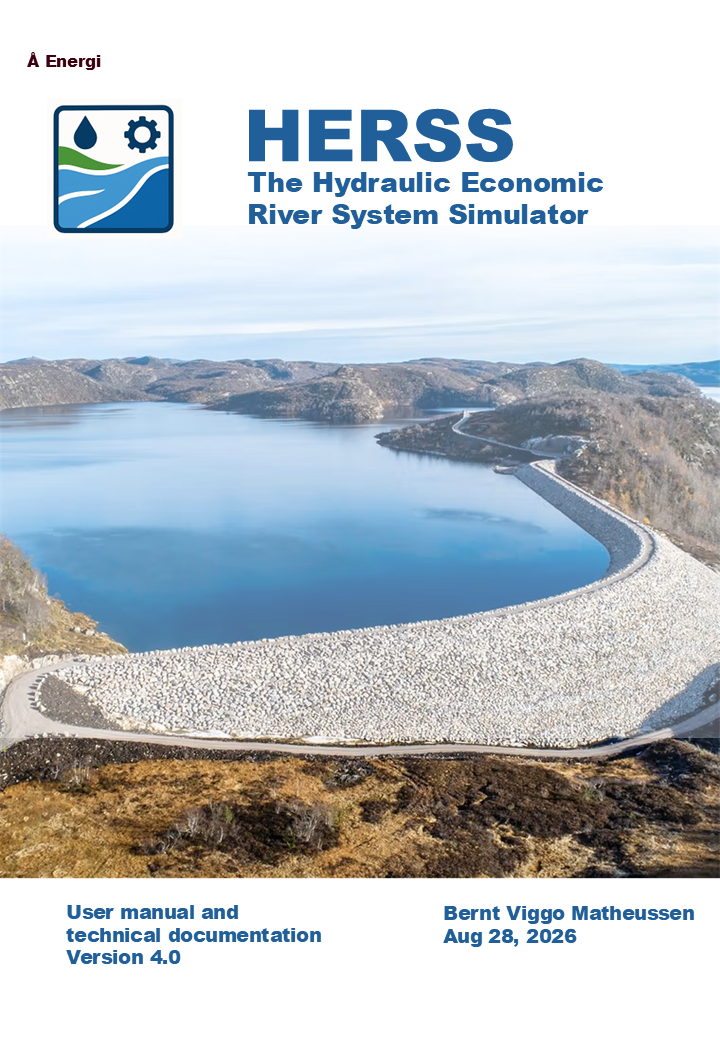
\includegraphics[width=\paperwidth, height=\paperheight, keepaspectratio=false]{./figures/frontpage}
			\clearpage
			\restoregeometry		
	\end{titlepage}
	\restoregeometry


	% --- roman numerals i, ii, iii ---
	\pagenumbering{roman}

	\input{license}
	% --- Preface ---
\newpage
\thispagestyle{empty}

\begin{center}
	\Large\textbf{Preface}
\end{center}

\vspace{2em}

Welcome to the user manual and technical documentation for the Hydraulic Economic River System Simulator (HERSS). HERSS is a lightweight and flexible simulation model for analysing the hydrology, hydraulics, and operation of regulated river systems, with particular emphasis on hydropower applications. The model can be used to simulate how water moves through a river system, how reservoirs and power stations interact, and how operational decisions and market conditions influence system behaviour over time.

This document is intended to provide enough information for users to get started with HERSS and to use the software effectively. A basic background in hydrology, river hydraulics, and hydropower is beneficial, but not strictly required. Some familiarity with working in a terminal on Ubuntu/Linux, or in Windows Subsystem for Linux (WSL), is also helpful when running the software and examples.

Regardless of your level of experience, the aim of this manual is to help you get up to speed with setting up simulations, understanding the model input and output, and using HERSS to analyse the dynamics of regulated river systems.

Please note that both the HERSS software and this documentation are still work in progress. The model is under active development, and some parts of the code, test datasets, and documentation may contain errors, inconsistencies, or incomplete descriptions. Not all details of the current HERSS version are yet fully documented, and in some cases the source code remains the most complete reference for how calculations are performed.

HERSS is developed as an open-source project, and contributions are welcome. Users and developers are encouraged to report issues, suggest improvements, and participate in further development of the model. The long-term goal of the HERSS project is to provide a fast, transparent, and adaptable simulation tool for a wide range of analyses of regulated river systems.
\newpage 


The HERSS model has been developed over several years, and many summer interns in Å Energi have used the software. The software has also been used in master thesis work, e.g. at the Univerity of Bergen. The timeline of major contributions in the HERSS project is shown in table \ref{tab:history}. 

\begin{table}[h]
	\centering
	\begin{tabular}{p{0.3\textwidth} p{0.65\textwidth}}
		\hline
		\textbf{Timeline} & \textbf{Changes/Contributions} \\
		\hline
		
		Spring 2023 &
		Initial code, testdata and documentation developed by BVM \\
		\\
		
		Summer 2023 &
		Development of testdata for Tovdalen Artifical Hydro Power System (TAHPS), by Kim Ly  \\
		\\
		
		
		Spring 2024 & GitHub repository established, by BVM \\
		\\
		
		Summer 2025 & 
		Main changes in the project: Added multi-generator support for up
		to six generators per power station. Added multi-temporal-
		resolution for simulation of varying timesteps. Added fast
		overflow. Added date check. Developed testing suite for HERSS
		functionality. This work was done by Ove Arstad. \\
		\\
		
		Spring 2026 & 
		Major upgrade and merging of new functionality (multi-resolution, multi-generator, new routing algorithm, etc). New documentation, plots, new test datasets, quality control, logging, etc. BVM May 2026. \\
		\\
		
		
		Summer 2026 &
		Terje Sandø implemented pumping, qmin, updated docs, minor bug fixes. New test riversystem. \\
				
		
		\hline
		
		
	\end{tabular}
	\caption{Timeline of the development and contributions to the HERSS project}
	\label{tab:history}
\end{table}

The HERSS project is supported by Å Energi (www.aenergi.no) \\

Bernt Viggo Matheussen, August 26, 2026.




	\tableofcontents
	
	\listoftables
	\listoffigures
	
	\clearpage
	\pagenumbering{arabic}
	\setcounter{page}{1}


	\chapter{Getting started}
	\label{chap:starting}
	This chapter helps you to get started. Make sure you have downloaded or 
	cloned the github repository (\texttt{https://github.com/berntmath/herss}). 
	
	\section{System Requirements} 
	
	The HERSS model is written in C++. It has been developed and tested using \cmd{g++} and Make,
	running on a Ubuntu operating system (20.04). It has also been tested on Ubuntu installed under
	the Windows Subsystem for Linux (WSL) and on standalone servers.
	The HERSS have successfully been compiled and run using \cmd{g++} version 9.3.0 and 9.4.0, and the
	GNU Make 4.2.1 program. The software has also been tested on Ubuntu 22.04 using \cmd{g++} 11.4.0.
	It compiled and ran without errors.
	The HERSS uses only standard C++ libraries and has no other dependencies. It should compile
	and run on most computers having a C++ compiler.
	The hardware requirements for the HERSS depend on how you intend to use the model. The test
	datasets that are part of the code has relatively low memory and CPU requirements and should run on
	almost any computer. 
	\newpage 
	
	
	\section{Installation instructions} 
	Download files from GitHub and unpack in a project directory. You should have a directory
	structure as shown in the figure below:
	
	\vspace{1em}
	
	
	\dirtree{%
		.1 herss/.
		.2 src/.
		.2 src\_tests/.
		.2 py\_src/.
		.2 doc/.
		.2 data/.
		.3 mini\_utahps\_daily/.
		.3 mini\_utahps\_hourly/.
		.3 res\_casc\_A/.
		.3 utahps\_daily/.
		.3 utahps\_hourly/.
		.3 utahps\_multires/.
		.2 README.md.
		.2 LICENSE.md.
	}	
	\vspace{1em}

	Open a terminal window and navigate into the \folder{src} directory. 
	Run \cmd{g++ --version} on the command line. 
	You should now see the version number and some additional text (similar to Figure \ref{fig:screen1}). 
	If it fails, you need to install \cmd{g++} on your system.
			
	\begin{figure}[h]
		\centering
		\includegraphics[width=0.9\textwidth]{./figures/screen1.png}
		\caption{Screenshot of terminal window after running the \cmd{g++} command.}
		\label{fig:screen1}
	\end{figure}

	
	Now type in \cmd{make --version} on the command line. 
	You should now see the version number and some additional text. 
	Your terminal window should look similar to Figure \ref{fig:screen1}. \\
		
	
	Open a terminal window and navigate into the \folder{src} directory.
	Run \cmd{make} on the command line. You should now se something similar to what is shown in Figure \ref{fig:screen2}. Look also for the files (\file{herss.exe} and \file{herss.so}). We need them later when we run the HERSS model from commandline or from within python.

	\begin{figure}[h]
		\centering
		\includegraphics[width=0.9\textwidth]{./figures/screen2.png}
		\caption{Screenshot of terminal window after running the \cmd{make} command.}
		\label{fig:screen2}
	\end{figure}
	
	
	\section{Running HERSS on the commandline}
	After you have downloaded and compiled the HERSS model you are now ready to use it. The HERSS
	model has no graphical user interface. It is run in a terminal/command window. We will now try
	to run a mini version of a riversystem (three nodes) using one of the datasets for 
	the Upper Tovdalen Artificial Hydro Power System (uTAHPS). 
	Navigate to the folder: \folder{./mini\_utahps\_hourly/}. You should see the folder \folder{./output/} and the following files:\\
	\begin{itemize}
		\item \file{actions.txt}
		\item \file{global.txt}
		\item \file{inflowseries.txt}
		\item \file{pricefile.txt}
		\item \file{start\_state.txt}
		\item \file{topology.txt}
	\end{itemize}	 
	 
	 Throughout this chapter, we will use the test dataset located in \file{mini\_uTAHPS\_hourly}.
	 Now run the HERSS model with the command \cmd{../../src/herss.exe global.txt}. 


	\begin{figure}[h]
	\centering
	\includegraphics[width=1.0\textwidth]{./figures/screen3.png}
	\caption{Screenshot of terminal window after running HERSS.}
	\label{fig:screen3}
	\end{figure}



	Congratulations! You have now completed your first simulation with the HERSS model.
	When HERSS started, it first read the global configuration file (\file{global.txt}). This file tells 
	the model which input files to use, where the input and output folders are located, 
	and which optional settings should be enabled during the run. After that, HERSS read 
	the main input files needed for the simulation. 
	These files includes the topology of the river system, 
	the inflow data, the price data, the action data, and the initial state file. 
	
	
	\begin{figure}[h]
	\centering
	\includegraphics[width=1.0\textwidth]{./figures/screen4.png}
	\caption{Screenshot of terminal/console showing the logfile.}
	\label{fig:screen4}
	\end{figure}
		
	
	At the end of the simulation, HERSS wrote the result files to the output folder and also created a log file:
	\file{herss\_3.0.01\_20260501.log}
	The log file contains useful information about the model run, 
	including startup messages, version information, progress messages, warnings, and possible error messages. 
	It can be helpful when checking that the simulation completed as expected or when diagnosing problems in the input files or model setup. \\
	
	If you use the command \cmd{more \file{herss\_3.0.01\_20260501.log}}, you will see something similar to Figure \ref{fig:screen4}.
	

	\section{Topology File and River System Structure}
	\label{sec:topo_start}

	The river system in this example is defined in the topology file \file{topology.txt}.
	The purpose of the topology file is to describe the physical structure of the 
	hydropower system and to provide the technical data needed for each node in the model. 
	In HERSS, a river system is built up from a sequence of nodes, where each node 
	represents a physical component such as a reservoir, a power station, or a river reach/channel.

	Figure~\ref{fig:mini} shows a schematic of the mini system used in this example. 
	The same structure is described in the topology file (\file{topology.txt}). 
	We have one reservoir named \texttt{Hjelle}. 
	This is connected to the powerstation \texttt{Svoletjonn}. 
	If the water level in the reservoir is above the highest 
	regulated water height (HRW), the water will flow into the channel called \texttt{Vanarosen}.
	In the powerstation \texttt{Svoletjonn}, the outflow from the station goes into the \texttt{Vanarosen} channel. 


	\begin{figure}[h]
		\centering
		\includegraphics[width=0.95\textwidth]{./figures/bilde5.pdf}
		\caption{Node structure and river topology of the mini uTAHPS system}
		\label{fig:mini}
	\end{figure}


	The topology file is divided into node blocks. Each block starts with a \texttt{NODE} line and ends with \texttt{ENDNODE}. The \texttt{NODE} line gives the node type, the node ID, and the node name. In this way, the file defines both the components of the river system and how they are connected.

	HERSS currently uses three main node types:

	\begin{itemize}
		\item \texttt{RESERVOIR}: a storage node where water is accumulated and released.
		\item \texttt{PSTATION}: a power station node where water is converted into hydropower production.
		\item \texttt{CHANNEL}: a river reach or routing node that transports water downstream.
	\end{itemize}

	Each node block contains the parameters that are relevant for that node type. For example, a reservoir node contain water levels, storage curves, and outlet definitions, while a power station node contains generator and efficiency data. A channel describes the hydraulic routing with traveltime, etc. 


   \section{Initial State File}
   
   The initial state file defines the hydraulic and operational state of the river system at the start of the simulation. In other words, it tells HERSS how much water is stored in reservoirs and channels, and what the initial condition of other dynamic components should be before the first time step is simulated. \\
   
   The initial state is given in the file \file{start\_state.txt}. This file is read during model initialization and provides the starting values needed to begin the simulation from a physically meaningful condition. The initial state file is organized by node type. Each relevant node is listed on a separate line together with the values needed to define its starting condition. For reservoirs, the file gives the initial filling as a fraction of the active storage range. In the mini uTAHPS example, the line
   
   \begin{verbatim}
   	NODE RESERVOIR 0 HJELLE 0.67
   \end{verbatim}
   
   \noindent means that reservoir 0, \texttt{HJELLE}, starts at a filling fraction of 0.67. This corresponds to 67\% of the active storage range between the lower regulated water level and the higher regulated water level. For power stations, the file gives the initial production state. In the example,
   
   \begin{verbatim}
   	NODE PSTATION 1 SVOLETJONN 0.0
   \end{verbatim}
   
   \noindent means that the power station \texttt{SVOLETJONN} starts with zero production. For channels, the file gives the initial storage in each linear reservoir used by the routing model. In the example,
   
   \begin{verbatim}
   	NODE CHANNEL 2 VANAROSEN 0.001 0.002 0.003
   \end{verbatim}
   
   \noindent means that channel 2, \texttt{VANAROSEN}, starts with three internal storage values, one for each linear reservoir in the channel cascade. The number of storage values must match the number of cascaded linear reservoirs defined in the topology file.
   

	\section{Time Series Input Data}

	In addition to topology and start state, HERSS needs time series input data to run the simulation. In the mini uTAHPS example, the time-dependent input is given in three files: \file{inflowseries.txt}, \file{pricefile.txt}, \file{actions.txt}. 
	
	\begin{figure}[h]
	\centering
	\includegraphics[width=0.85\textwidth]{./figures/inflowseries_gmt.pdf}
	\caption{Input timeseries (inflow, price, and actions) for the mini uTAHPS}
	\label{fig:mini_inputseries}
	\end{figure}
	
	Together, these files describe how much water enters the system, what the electricity price is at each time step, and how the power station is operated during the simulation period. The action variable is a control signal with values between 0.0 and 1.0. It determines the flow through the power station as a fraction of the maximum flow capacity. A value of 0.0 means that the station is off, a value of 1.0 means full operation, and intermediate values represent partial operation. Figure~\ref{fig:mini_inputseries} shows a timeseries plot of the input testdata.

	\section{Output Data from HERSS}

	After a simulation has finished, HERSS writes a set of output files to the output folder. 
	These files contain both aggregated results for the full river system and more detailed 
	results for individual nodes such as reservoirs, power stations, and channels. Together, 
	the output files make it possible to inspect the hydraulic behaviour of the system, 
	evaluate operational performance, and analyse the economic results of the simulation.

	\begin{figure}[h]
		\centering
		\includegraphics[width=0.85\textwidth]{./figures/outputseries.pdf}
		\caption{Output timeseries for the mini uTAHPS}
		\label{fig:mini_outputseries}
	\end{figure}


	In practice, the output data can be used to make time series plots of selected variables, for example reservoir levels, hydropower production, and outflow from channels. These plots are often the most convenient way to understand how the simulated river system behaves over time. Figure \ref{fig:mini_outputseries} illustrates the reservoir levels, power production and channel flow for the uTAHPS. Note how the reservoir level changes as a function of inflow (see Fig. \ref{fig:mini_inputseries}) and outflow (production, MWh).
	
	The downstream channel (node 2) in the mini uTAHPS system represents routing of water from the power station further downstream. The channel node also receives overflow water from the reservoir (Hjelle). In the simulation, the channel does not simply pass inflow directly to the outlet at the same time step. Instead, the flow is delayed and smoothed as it moves through the channel. In HERSS, the channel routing is represented by a cascade of linear reservoirs. This gives a simple but effective description of how water is temporarily stored and released as it travels downstream. For the mini uTAHPS example, the channel is configured with three cascaded linear reservoirs and a travel time parameter of four hours. Together, these settings control how strong the delay and attenuation become.
	

	This behaviour can be seen in the time series plot (Fig. \ref{fig:mini_outputseries})) of channel inflow and channel outflow. The inflow curve shows the water entering the channel from upstream, while the outflow curve shows the water leaving the channel after routing through the channel model. In general, the outflow does not respond instantaneously to changes in inflow. Instead, peaks in inflow appear later in time at the outlet. This is the routing delay.

	At the same time, the outflow signal is usually smoother than the inflow signal. Sharp peaks in inflow tend to become lower and broader in the outflow series. This effect is known as attenuation. Physically, it reflects temporary storage and redistribution of water inside the channel reach. More on this in chapter \ref{chap:structure}


	\subsection{Overview of the Output Files}

	The most important output files are written to the output folder after each model run. Typical files include:

	\begin{itemize}
		\item \file{riversystem\_<systemname>\_output.txt}
		\item \file{reservoirs\_<systemname>\_out.txt}
		\item \file{outstate.txt}
		\item optional node output files such as \file{node0\_HJELLE.txt}, \file{node1\_SVOLETJONN.txt}, and \file{node2\_VANAROSEN.txt}
	\end{itemize}

	The exact names depend on the system name given in the global configuration file and on whether node-level output has been enabled.

	\subsection{Aggregated River System Output}

	The file \file{riversystem\_<systemname>\_output.txt} contains summary information for the entire river system. This file includes information about the nodes in the system, the remaining water in the different parts of the river network, and the global water balance.

	In addition, this file contains important aggregated economic quantities, such as total income, total cost, total profit, the estimated value of remaining water, and the final value function. These results provide a compact summary of the overall performance of the simulated system over the full time horizon.

	\subsection{Reservoir Output}

	The file \file{reservoirs\_<systemname>\_out.txt} contains time series of reservoir filling for all reservoir nodes in the system. The values are written as reservoir fractions, typically denoted by \texttt{fr}, for each simulation time step. This file is particularly useful for plotting reservoir levels over time and for checking whether the reservoirs are being drawn down or refilled as expected during the simulation period.

	\subsection{Node-Level Output}

	If node-level output is enabled, HERSS writes one file for each node in the system. These files contain the most detailed simulation results and are often the most useful outputs for plotting and interpretation.

	For a reservoir node, the output file typically contains variables such as:

	\begin{itemize}
		\item inflow,
		\item upstream inflow,
		\item reservoir storage,
		\item reservoir water level,
		\item reservoir filling fraction,
		\item tunnel flow,
		\item hatch flow,
		\item overflow, and
		\item total outflow.
	\end{itemize}

	For a power station node, the output file typically contains variables such as:

	\begin{itemize}
		\item upstream inflow,
		\item action values,
		\item total outflow,
		\item head,
		\item power production,
		\item income,
		\item operating cost, and
		\item profit.
	\end{itemize}

	For a channel node, the output file typically contains variables such as:

	\begin{itemize}
		\item upstream inflow,
		\item channel storage,
		\item total outflow, and
		\item possible minimum-flow related costs.
	\end{itemize}

	These node-level files are well suited for making time series plots of selected variables, for example reservoir levels, hydropower production, or outflow from a downstream channel.

	\subsection{State Output}

	HERSS also writes an output state file, typically named \file{outstate.txt}. This file contains the simulated end state of the system after the last time step. It can be used as a restart state for a later simulation, making it possible to continue from the final condition of a previous model run.


	\subsection{Use of the Output Data}
	The output data from HERSS can be used for several purposes:

	\begin{itemize}
		\item checking that the simulation behaved as expected,
		\item verifying water balances and system routing,
		\item plotting time series of key variables,
		\item comparing different operational strategies, and
		\item evaluating the hydraulic and economic performance of the system.
		\item long term planning analysis
		\item design of new systems
		\item optimization of daily power production and reservoir management
	\end{itemize}

	For the simple uTAHPS example, useful plots include reservoir level in the Hjelle reservoir, production from the power station, and outflow from the downstream channel. Such plots provide a clear and intuitive way to interpret the model results. \\
	
	That's it!. Now you have a basic understanding of the HERSS model, 
	how to run it, and what results it produces. \\
	
	The rest of this document will focus on three parts: model structure, more tutorials and testdata. 

	\newpage 



	%-------------------------------------------------------------------------------------
	%-------------------------------------------------------------------------------------
	%-------------------------------------------------------------------------------------


	\chapter{Model structure}
	\label{chap:structure}

	HERSS represents a regulated river system as a network of nodes, where each node corresponds to a physical component such as a reservoir, a power station, or a river channel. Every node has a unique identifier and belongs to one of the supported node types. Water enters a node from upstream, is processed according to the physical behavior of that node type, and is then routed to one or more downstream nodes, stepping forward in time until the end of the simulation period.

	This node-based approach makes it straightforward to represent river systems of varying complexity, from a simple single-reservoir system to large networks with many reservoirs, power stations, and channels arranged in branched or cascaded configurations. This chapter describes the supported node types, how they are connected, and what physical processes each one represents.
		
	Figure~\ref{fig:model_structure} shows a schematic of a more complex river network, illustrating how different node types can be combined to represented a realistic hydropower system.
	
	\begin{figure}[h]
		\centering
		\includegraphics[width=0.75\textwidth]{./figures/utahps.pdf}
		\caption{Schematic of a hydropower river system represented as a network of nodes in HERSS.}
		\label{fig:model_structure}
	\end{figure}
	
	\section{Node Topology and ordering}
	The order in which nodes are defined in the topology file determines the order in which they are simulated at each time step. Water is routed from the most upstream node towards the most downstream node in sequence. It is therefore important that the topology file correctly reflects the physical layout and connectivity of the river system. 
	
	The topology file defines the river system as a directed acyclic graph (DAG) of nodes, where each node represents either a reservoir, a power station, a channel reach, or a pump (Section~\ref{subsec:pump}). Each node is assigned a unique integer identifier (\texttt{IDNR}), starting at zero. The calculation order in HERSS is determined entirely by the node numbering: at each time step, nodes are simulated in ascending order of their \texttt{IDNR}, from node~$0$ to node~$N-1$, where $N$ is the total number of nodes.
	
	This sequential ordering imposes a strict requirement on how nodes are numbered in the topology file: \textbf{all upstream nodes must be assigned lower identifiers than the downstream nodes they drain into, with only one exception for pumped hydro}. In other words, water can only flow from a node with a lower \texttt{IDNR} to a node with a higher \texttt{IDNR}. When a node is simulated at time step~$t$, it reads the upstream inflow (\texttt{up\_inflow}) that has already been written by all upstream nodes in the same time step. It then computes its own outflow and adds it to the \texttt{up\_inflow} accumulator of its downstream node, which has not yet been simulated in that time step.
	
	A concrete consequence is illustrated below. Consider a cascaded system with three nodes:
	
	\begin{itemize}
		\item Node~0: upstream reservoir
		\item Node~1: power station, receives discharge from node~0
		\item Node~2: downstream channel or reservoir, receives discharge from node~1
	\end{itemize}
	
	At each time step, the simulation loop processes node~0, node~1, and node~2 in that order. Node~0 computes its outflow and writes it to \texttt{node[1].up\_inflow[t]}. Node~1 reads this value, computes its own turbine discharge, and writes it to \texttt{node[2].up\_inflow[t]}. Node~2 then uses the accumulated inflow for its own computation.

	
	If a node receives water from multiple upstream sources (e.g.\ a confluence/junction), all contributing upstream nodes must have lower identifiers than the receiving node. Branching topologies, such as a reservoir with both a tunnel outlet and an overflow outlet leading to different downstream nodes, are supported, but all downstream nodes must again have higher identifiers than the source node.
	
	A \texttt{PUMP} node, representing a Pumped Storage Hydropower (PSH) facility (Section~\ref{subsec:pump}) is the one exception to the sequential ordering rule: since it moves water against the normal flow direction, both \texttt{PUMP\_SOURCE\_IDNR} and \texttt{PUMP\_TARGET\_IDNR} must be \emph{higher} than the pump's own \texttt{IDNR}.
	
	\subsection*{Numbering Guidelines}
	
	The following guidelines should be followed when constructing a topology file:
	
	\begin{enumerate}
		\item Start numbering at zero (\texttt{IDNR = 0}) for the most upstream node in the system.
		\item Assign identifiers in strictly increasing order in the downstream direction.
		\item At confluences, ensure that \emph{all} contributing nodes have identifiers lower than the receiving node.
        \item When placing a \texttt{PUMP} node, plan it ahead so it is given a lower \texttt{IDNR} than both its source and target reservoirs.
		\item The last node in the topology (highest \texttt{IDNR}) is typically the most downstream node, for example the ocean or a boundary channel with no downstream connection (indicated by a downstream identifier of \texttt{-9} in the topology file).
	\end{enumerate}
	
	HERSS does \emph{not} automatically sort or validate the topological order of nodes at runtime. It is the responsibility of the model user to ensure that node identifiers reflect a valid upstream-to-downstream ordering. An incorrect ordering will lead to erroneous water routing, because a downstream node may be simulated before all its upstream contributions have been computed for the current time step, resulting in those contributions being applied one time step too late.
	\newpage

	\section{Node Types}
	\label{sec:nodetypes}

	HERSS currently supports four node types:

	\begin{itemize}
		\item \textbf{Reservoir}: a storage node representing a regulated lake or impoundment. The reservoir receives inflow, stores water, and releases it through one or more outlets to downstream nodes.
		\item \textbf{Power station}: a node representing a hydropower plant. The power station receives water from an upstream reservoir, generates electricity from the turbine discharge, and passes the discharged water downstream.
		\item \textbf{Channel}: a routing node representing a river reach or transport element. The channel receives water from upstream and routes it downstream with delay and attenuation.
        \item \textbf{Pump}: a node representing a pumped-storage hydropower (PSH) facility, using electricity to move water from a source reservoir to a target reservoir.
	\end{itemize}

	Each node type is described in detail in the following subsections.

	\subsection{Reservoir}
	\label{subsec:reservoir}

	The node type \texttt{RESERVOIR} models a hydro power reservoir. For each reservoir the user must supply a piecewise-linear \emph{reservoir curve} that maps water surface elevation (meters above sea level, masl) to stored volume (Mm$^3$). A minimum of two points is required, but minimum four points are recommended. The curve must span from below the Lowest Regulated Water (LRW) level to above the Highest Regulated Water (HRW) level, and ideally extend somewhat beyond both limits to avoid extrapolation errors during extreme events. \\

	A reservoir may have up to four independent outlets, each sending water to a specified
	downstream node identified by its \texttt{IDNR}. All outlets are optional except overflow,
	which is always active. Within each time step, outlets are evaluated in the following fixed
	order: tunnel, hatch, automatic minimum-flow release, and finally overflow. A schematic of the
	outlet types is shown in Figure \ref{fig:reservoir}.
	

	\begin{description}
	
	\item[Tunnel (\texttt{OUTLET\_TUNNEL})] The primary production outlet, connecting the
	reservoir to a downstream power station node. The reservoir passes its current water
	surface elevation to the power station so that the net hydraulic head can be computed.
	The discharge through the tunnel is determined by the power station's action variable,
	not by the reservoir directly.
	
	\item[Hatch (\texttt{OUTLET\_HATCH})] A controllable gate, typically releasing water to a
	downstream channel. The discharge is a linear interpolation between a minimum flow
	$Q_\mathrm{min}$ and a maximum flow $Q_\mathrm{max}$, controlled by the action
	variable $a \in [0,\,1]$:
	$$Q_\mathrm{hatch} = Q_\mathrm{min} + a\,(Q_\mathrm{max} - Q_\mathrm{min})$$
	The hatch only operates when the reservoir level exceeds the sill elevation
	(\texttt{hatch\_masl}). An action time series must be supplied for nodes with an
	active hatch outlet.
	
	\item[Automatic minimum-flow release (\texttt{OUTLET\_AUTO\_QMIN})] A seasonally
	scheduled release that operates independently of the optimisation action. It is used
	to enforce regulatory minimum-flow requirements directly from the reservoir, for
	example a fixed environmental flow obligation. Up to five seasonal periods may be
	defined, each with its own minimum discharge.

    When \texttt{OUTLET\_AUTO\_QMIN} is used, HERSS expect the following arguments:
    \begin{verbatim}
    OUTLET_AUTO_QMIN <nr_periods> <downstream_idnr> <outlet_masl>
    <start date DD.MM> <end date DD.MM> <Qmin m3/s>
    ...
    \end{verbatim}
    where \texttt{nr\_periods} is the integer describing the number of defined periods listed
    below (Maximum number of 5). Set \texttt{nr\_periods} to a non-positive value (e.g.\
    \texttt{-9999}) to disable \texttt{OUTLET\_AUTO\_QMIN} entirely. At most one of the defined periods may
    cross the turn of the year (e.g.\ \texttt{01.10 31.03}). HERSS will return warnings for days in the year which is not covered in the defined periods.  Overlapping periods will be ignored, and only the overlapping period with the first start date will be used. The minimum-flow release hatch is placed at \texttt{outlet\_masl}, and water below this level will not be available for release.
	
	\item[Overflow (\texttt{OVERFLOW\_CURVE})] Uncontrolled spillage over the dam crest,
	described by a piecewise-linear curve mapping reservoir elevation to overflow discharge
	[m$^3$/s]. Overflow is computed last, after all controlled outlets have been evaluated,
	and drains to a specified downstream node. Every reservoir must have an overflow curve
	defined.
	
	\end{description}


	\begin{figure}[h]
		\centering
		\includegraphics[width=0.7\textwidth]{./figures/reservoir.pdf}
		\caption{Node type reservoir with the four outlet options.}
		\label{fig:reservoir}
	\end{figure}

	\newpage 



	\subsubsection{Reservoir geometry}

	As an alternative to specifying a measured volume--elevation curve (\texttt{RESERVOIR\_CURVE}), the reservoir shape can be described by a simple parametric geometry  (\texttt{RESERVOIR\_GEOMETRY})  . This option is activated by supplying the five keywords \texttt{RESERVOIR\_GEOMETRY}, \texttt{WIDTH\_M}, \texttt{LENGTH\_M}, \texttt{THETA}, and \texttt{BOTTOM\_MASL} in the reservoir node block. The two representations are mutually exclusive; using both in the same node will cause a model error.

	\paragraph{Geometric model}

	The reservoir is approximated as a rectangular basin with uniform cross-section along its length. The side slopes are parameterised by the angle $\theta$, measured from the horizontal. A derived slope term is computed once at initialisation:

	\begin{figure}[h]
		\centering
		\includegraphics[width=0.7\textwidth]{./figures/reservoir1.pdf}
		\caption{Reservoir with parametric geometry}
		\label{fig:reservoir_geo}
	\end{figure}


	\begin{equation}
		s = \tan\!\left(\frac{(90 - \theta)\,\pi}{180}\right)
	\end{equation}

	The stored volume at water surface elevation $z$ [m.a.s.l.] is then:

	\begin{equation}
		V(z) = \frac{h \cdot (s + W) \cdot L}{10^6} \quad [\text{Mm}^3]
	\end{equation}

	\noindent where $h = z - z_\text{bottom}$ is the depth above the reservoir floor and $W$, $L$ are the bottom width and length respectively. The inverse relation, used to convert a stored volume back to a water surface elevation, is:

	\begin{equation}
		z = z_\text{bottom} + \frac{V \times 10^6}{L \cdot (s + W)}
	\end{equation}

	Both relations are linear in $h$ (or $V$), making the geometry computationally inexpensive compared to table interpolation on a measured curve.

	\paragraph{Physical interpretation of $\theta$}

	The angle $\theta$ describes the inclination of the valley sides:
	\begin{itemize}
		\item $\theta \to 90°$: nearly vertical side walls, approximately rectangular cross-section ($s \to 0$).
		\item $\theta \to 0°$: very gently sloping valley ($s \to \infty$, large effective width per unit depth).
	\end{itemize}
	A value of $\theta = 20°$ represents a moderately V-shaped valley.

	\paragraph{Topology file syntax}

\begin{verbatim}
	RESERVOIR_GEOMETRY
	WIDTH_M    1000
	LENGTH_M   1000
	THETA      20
	BOTTOM_MASL  745.0
\end{verbatim}

\noindent The parameters are:
\begin{center}
	\begin{tabular}{lll}
		\hline
		Keyword & Type & Description \\
		\hline
		\texttt{WIDTH\_M}     & float & Bottom width of the reservoir [m] \\
		\texttt{LENGTH\_M}    & float & Length of the reservoir [m] \\
		\texttt{THETA}        & float & Side-slope angle from horizontal [degrees], $0 < \theta < 90$ \\
		\texttt{BOTTOM\_MASL} & float & Elevation of the reservoir floor [m.a.s.l.] \\
		\hline
	\end{tabular}
\end{center}

\paragraph{Constraints and notes}

\begin{itemize}
	\item \texttt{RESERVOIR\_GEOMETRY} and \texttt{RESERVOIR\_CURVE} are mutually exclusive; specifying both will cause a model error.
	\item \texttt{WIDTH\_M} and \texttt{LENGTH\_M} must be positive; \texttt{THETA} must satisfy $0 < \theta < 90$.
	\item \texttt{BOTTOM\_MASL} must be non-negative and physically plausible.
	\item The geometry-based volume--elevation relationship is linear, which is a simplification. For reservoirs with strongly irregular bathymetry a measured \texttt{RESERVOIR\_CURVE} is more accurate.
\end{itemize}




	\subsubsection{Fast Overflow}
	\label{subsubsec:fast_overflow}

	By default, overflow is computed by interpolating the overflow curve at the current reservoir
	elevation. For large time steps, or when simulation speed is critical, the \texttt{FAST\_OVERFLOW}
	option can be enabled. With this setting, overflow is calculated simply as the volume above
	\texttt{HRW}, without interpolating the overflow curve:

	$$Q_\mathrm{overflow} = \max\!\left(V - V_\mathrm{HRW},\; 0\right)$$

	This avoids the curve look-up and is numerically more stable for coarse time steps. To enable
	it, set \texttt{FAST\_OVERFLOW TRUE} for the relevant reservoir in the topology file.




	\subsubsection{Spillway}

	A spillway is a fixed-crest overflow structure that releases water from a reservoir once the water surface elevation exceeds the crest level. It is one of two mutually exclusive methods available for modelling uncontrolled overflow; the other is the \texttt{OVERFLOW\_CURVE}. Both methods cannot be active simultaneously for the same reservoir node.

	\paragraph{Discharge formula}

	The spillway discharge is computed using the standard broad-crested weir formula:

	\begin{equation}
		Q = C \cdot L \cdot H^{3/2}
		\label{eq:spillway}
	\end{equation}

	\noindent where:
	\begin{itemize}
		\item $Q$ \quad is the spillway discharge [m$^3$/s],
		\item $C$ \quad is the dimensionless discharge coefficient [--],
		\item $L$ \quad is the crest length [m],
		\item $H = z_\text{res} - z_\text{crest}$ \quad is the head above the spillway crest [m], computed as the difference between the current reservoir water surface elevation $z_\text{res}$ and the fixed crest elevation $z_\text{crest}$, both in metres above sea level (m.a.s.l.).
	\end{itemize}

	Discharge is zero whenever $z_\text{res} \leq z_\text{crest}$.

	\paragraph{Volume limitation}

	The computed discharge volume per time step is capped to prevent the reservoir from draining below the spillway crest level:

	\begin{equation}
		\Delta V_\text{overflow} = \min\!\left(Q \cdot \Delta t,\; V_\text{res} - V_\text{crest}\right)
	\end{equation}

	\noindent where $V_\text{res}$ is the current stored volume and $V_\text{crest}$ is the reservoir volume corresponding to $z_\text{crest}$. This ensures numerical stability with large time steps.

	\paragraph{Topology file syntax}

	The spillway is configured in the topology file with a single line inside the reservoir node block:

	\begin{verbatim}
		SPILLWAY  downstream_idnr  C  L  spillway_level_masl
	\end{verbatim}

	\noindent The parameters are:
	\begin{center}
		\begin{tabular}{lll}
			\hline
			Field & Type & Description \\
			\hline
			\texttt{downstream\_idnr}      & integer & Node ID receiving the spillway discharge \\
			\texttt{C}                     & float   & Discharge coefficient \\
			\texttt{L}                     & float   & Crest length [m] \\
			\texttt{spillway\_level\_masl} & float   & Crest elevation [m.a.s.l.] \\
			\hline
		\end{tabular}
	\end{center}

	The downstream node must not be the same as the reservoir itself. The crest elevation $z_\text{crest}$ may be set below the high reservoir water level (HRW), in which case spillway discharge can occur while the reservoir is still below its design maximum.

	\paragraph{Constraints and notes}

	\begin{itemize}
	\item \texttt{SPILLWAY} and \texttt{OVERFLOW\_CURVE} are mutually exclusive for a given reservoir; specifying both will cause a model error.
	\item The discharge coefficient $C$ must be in the range $(0,\,100]$ and the crest length $L$ must be positive.
	\item The crest elevation must be a physically plausible value (positive and below the summit of Mount Everest, used internally as an upper sanity bound).
	\item If the \texttt{FAST\_OVERFLOW} flag is set to \texttt{TRUE}, the normal weir formula is bypassed and the overflow volume is set directly to the volume exceeding HRW. This is a simplified, computationally cheaper approximation and is not recommended when accurate spillway hydraulics are required.
	\end{itemize}




	\subsubsection{LRW Penalty Cost}
	\label{subsubsec:lrw_penalty}

	If the reservoir level falls below \texttt{LRW}, a cost is incurred that is proportional to
	both the depth of the violation and the length of the time step:

	$$C_\mathrm{LRW} = p \cdot \frac{\Delta t}{3600} \cdot \left(\mathrm{LRW} - h\right)$$

	where $p$ is the penalty parameter \texttt{RES\_PENALTY}, $\Delta t$ is the time step in
	seconds, and $h$ is the current water surface elevation [masl]. The linear dependence on the
	depth of violation ensures a smooth, differentiable cost function that provides a meaningful
	gradient signal for optimization algorithms: a deeper violation produces a proportionally
	larger cost. Note that aggressive actions can impact this. 

	\newpage


	\subsection{Powerstation}
	\label{subsec:powerstation}

	The \texttt{PSTATION} node models a hydropower power station. Unlike the reservoir node, the
	power station cannot store water. All water that enters the node in a given time step must leave it
	in the same time step via the downstream connection (\texttt{DOWNLINK\_IDNR}).

	A power station node receives water exclusively through its upstream reservoir tunnel
	connection. The upstream reservoir passes its water surface elevation at the start and end of
	the time step to the power station, which uses these values to compute the available hydraulic
	head (Hnetto). Figure \ref{fig:powerstation} illustrates how a powerstation is connected to a reservoir through a tunnel. 

	\begin{figure}[h]
		\centering
		\includegraphics[width=0.7\textwidth]{./figures/powerstation.pdf}
		\caption{Node type powerstation.}
		\label{fig:powerstation}
	\end{figure}

	\subsubsection{Hydraulic Head and Power Calculation}

	The gross hydraulic head is computed as the average reservoir elevation over the time step,
	minus the turbine elevation:

	$$
		H_\mathrm{brutto} = \frac{h_\mathrm{start} + h_\mathrm{end}}{2} - h_\mathrm{turbine}
	$$

	where $h_\mathrm{start}$ and $h_\mathrm{end}$ are the reservoir water surface elevations
	[masl] at the beginning and end of the time step respectively, and $h_\mathrm{turbine}$ is
	the turbine centreline elevation (\texttt{POWSTAT\_MASL}) [masl].

	Head losses in the penstock are modelled using a quadratic loss formula:

	\begin{equation}
	    \Delta H = k \cdot Q^2
        \label{eq:Headloss}
	\end{equation}
	

	where $k$ is the head loss coefficient (\texttt{HEADLOSSCOEF}) and $Q$ is the discharge
	[m$^3$/s]. The net head is then:


	\begin{equation}
	    H_\mathrm{netto} = H_\mathrm{brutto} - \Delta H
        \label{eq:Head_net}
	\end{equation}

	Mechanical power output for each generator is:

	\begin{equation}
	    P = \eta_\mathrm{turbine}(Q) \cdot \eta_\mathrm{generator} \cdot \rho g \cdot H_\mathrm{netto} \cdot Q \quad \text{[MW]}
        \label{eq:Gen_Mech_power}
	\end{equation}
	

	where $\eta_\mathrm{turbine}(Q)$ is the turbine efficiency at the current discharge, read from
	the turbine efficiency curve, and $\eta_\mathrm{generator}$ is the static generator efficiency.
	Energy produced in the time step is:

	$$
	E = P \cdot \frac{\Delta t}{3600} \quad \text{[MWh]}
	$$


	\subsubsection{Generators and Turbine Efficiency Curve}
	A power station may have one or more generators (\texttt{NR\_GENERATORS}, maximum
	\texttt{MAX\_NR\_GENERATORS}). Each generator has its own:

	\begin{itemize}
		\item A piecewise-linear \emph{turbine efficiency curve} (\texttt{TURBINE\_CURVE})
		mapping discharge [m$^3$/s] to efficiency [\%].
		\item A maximum discharge (\texttt{GENERATOR\_MAX\_DISCHARGE}) [m$^3$/s].
		\item An action variable $a \in [0, 1]$, where the actual discharge is
		$Q = a \cdot Q_\mathrm{max}$.
	\end{itemize}

	Each generator requires a corresponding action column in the actions input file. \newline
	
	
	\subsubsection{Uniform normalised turbine efficiency curve}
	
	As a faster alternative to the general \texttt{TURBINE\_CURVE}, a generator's efficiency can be specified using a uniformly-sampled normalised curve via the \texttt{UNIFORM\_NORMALIZED\_CURVE} keyword. Because the sample points are equally spaced in normalised discharge, the correct table entry can be found by direct index calculation rather than a binary search, making simulation runs significantly faster when many function evaluations are performed.
	
	\paragraph{Definition}
	
	The curve is defined by exactly $N = 11$ efficiency values $\eta_k$ sampled at normalised discharges
	
	\begin{equation}
		Q_n^{(k)} = \frac{k}{N-1}, \quad k = 0, 1, \ldots, N-1
	\end{equation}
	
	\noindent i.e.\ at $Q_n \in \{0.0,\, 0.1,\, 0.2,\, \ldots,\, 1.0\}$, where the normalised discharge is defined as
	
	\begin{equation}
		Q_n = \frac{Q}{Q_\text{max}}
	\end{equation}
	
	\noindent and $Q_\text{max}$ is the \texttt{GENERATOR\_MAX\_DISCHARGE} for that generator.
	
	\paragraph{Interpolation at runtime}
	
	Given an actual discharge $Q$, the efficiency is evaluated by:
	
	\begin{align}
		Q_n &= Q \;/\; Q_\text{max} \\
		i   &= \lfloor Q_n \cdot (N-1) \rfloor \\
		t   &= Q_n \cdot (N-1) - i \\
		\eta &= \eta_i + t\,(\eta_{i+1} - \eta_i)
	\end{align}
	
	\noindent This is a simple linear interpolation with $O(1)$ index access. The returned fractional efficiency is $\eta / 100$.
	
	\paragraph{Topology file syntax}
	
	The keyword replaces \texttt{TURBINE\_CURVE} inside a \texttt{GENERATOR} block and must always be followed immediately by \texttt{GENERATOR\_MAX\_DISCHARGE}:
	
	\begin{verbatim}
		GENERATOR 0
		UNIFORM_NORMALIZED_CURVE 11
		0.0   0.0
		0.1  50.0
		0.2  75.0
		0.3  86.0
		0.4  90.0
		0.5  92.0
		0.6  91.5
		0.7  90.0
		0.8  88.0
		0.9  85.0
		1.0  82.0
		GENERATOR_MAX_DISCHARGE 4.0
	\end{verbatim}
	
	\noindent The first column is the normalised discharge $Q_n$ and is for human readability only; the parser reads only the second column (efficiency in percent). The integer after \texttt{UNIFORM\_NORMALIZED\_CURVE} must equal $N = 11$; any other value will cause a model error.
	
	\paragraph{Constraints and notes}
	
	\begin{itemize}
		\item \texttt{UNIFORM\_NORMALIZED\_CURVE} and \texttt{TURBINE\_CURVE} are mutually exclusive within a single generator block.
		\item Exactly 11 efficiency values must be provided, corresponding to $Q_n = 0.0, 0.1, \ldots, 1.0$.
		\item Efficiency values are given in percent [\%]; they are divided by 100 internally before use.
		\item If the discharge passed to the efficiency function is below $10^{-6}$ m$^3$/s the function returns zero without consulting the curve.
		\item Discharges above \texttt{GENERATOR\_MAX\_DISCHARGE} are treated as an error; the simulation will abort with a diagnostic message.
	\end{itemize}
	

    \subsubsection{Headloss in the tunnel}
    The \texttt{HEADLOSSCOEF} k in eq. (\ref{eq:Headloss}) which is used to estimate head loss eq. (\ref{eq:Head_net}) and eq. (\ref{eq:Gen_Mech_power}) is derived from the Darcy Weisbach equation: 

    \begin{equation}
        h_f=f_d \cdot \frac{LV^2}{2gD}
        \label{Darcy_Weisbach}
    \end{equation}
    where $f_d$ is the dimensionless Darcy friction factor, $L$ is the tunnel length, $V$ is the speed of water, $g$ is the gravitational acceleration and $D$ is the tunnel diameter. 

    Substituting $V=\frac{Q}{A}$ into eq. (\ref{Darcy_Weisbach}) and comparing the resulting expression with eq. (\ref{eq:Headloss}) yields the tunnel head loss coefficient

    \begin{equation}
        k = \frac{f_d L}{2 g D A^2},
        \label{eq:HEADLOSSCOEF}
    \end{equation}

    depending on the Darcy friction factor, tunnel length, and the tunnel diameter and cross-sectional area. The Darcy friction factor may be found in tables for different surface roughnesses.

	\subsubsection{Penstock Configuration}

	Two penstock configurations are supported, selected with \texttt{SHARED\_PENSTOCK}:

	\begin{description}
		\item[\texttt{SHARED\_PENSTOCK TRUE}] All generators draw from a single common penstock.
		Head loss is computed from the combined total discharge of all generators, and the
		resulting net head applies equally to all.
	
		\item[\texttt{SHARED\_PENSTOCK FALSE}] Each generator has its own independent penstock.
		Head loss and net head are computed separately for each generator based on its
		individual discharge.
	\end{description}


	\subsubsection{Minimum Discharge}

	The parameter \texttt{POWSTAT\_MIN\_DISCHARGE} defines the minimum operational discharge
	[m$^3$/s] of the power station. If the total discharge falls below this threshold (but is
	greater than zero), a warning is issued. This is currently implemented as a soft constraint:
	the simulation continues but flags the violation in the log. The minimum discharge is used
	primarily to indicate a technically meaningful lower operating limit for the turbines.

    \subsubsection{Local Energy Equivalent (\texttt{LOCAL\_ENERGY\_EQUIVALENT})}
    The \texttt{LOCAL\_ENERGY\_EQUIVALENT} [kWh/m$^3$] is a power station specific factor used
    to convert the water volume stored above LRW in the reservoirs upstream of it into an estimate of the remaining producible energy. It is a static coefficient and should be estimated using
    representative values for the head and efficiency of each power station and its reservoir.
    
    The energy equivalent is used together with \texttt{RESTPRICE} in the input pricefile to
    estimate the value of the water remaining in the river system at the end of the simulation.

	\subsubsection{Automatic Minimum Flow (\texttt{AUTO\_QMIN})}

	If \texttt{AUTO\_QMIN} is set to a positive value, the power station enforces a minimum flow
	through the turbines regardless of the action variable. This is intended for situations where
	a regulatory minimum flow must pass through the power station itself, rather than being
	bypassed to a channel. If the action-based discharge falls below \texttt{AUTO\_QMIN}, the
	flow is raised to meet it.

	\subsubsection{Start and Stop Costs}

	A start/stop cost (\texttt{POWSTAT\_STARTSTOP}) [EUR] is incurred each time a generator
	transitions between the off state ($a = 0$) and the on state ($a > 0$), or vice versa. The
	cost is split equally between the start event and the stop event, so each transition
	contributes $\texttt{POWSTAT\_STARTSTOP} / 2$ to the total cost. This penalty discourages
	frequent cycling, which is physically costly in real plant operation.

	\subsubsection{Aggressive Action Penalty}

	If the requested discharge in a time step exceeds the available water volume in the upstream
	reservoir, the power station discharge is forced to zero and a large penalty cost is applied.
	This mechanism can be useful in e.g. optimization. It denies requesting physically impossible discharges while
	still providing a strong gradient signal to drive the solution away from infeasible regions.
	\newpage 















	\subsection{Channel}
	\label{subsec:channel}

	The \texttt{CHANNEL} node models the transport of water through a river reach between two
	nodes. It introduces a travel time delay and attenuation of the flood wave, representing the
	physical processes of translation and dispersion in a natural watercourse. Unlike the power
	station, the channel produces no electricity and carries no economic value on the water
	stored within it.

	A channel node receives water from its upstream neighbour through the standard
	\texttt{up\_inflow} mechanism and routes it to a single downstream node specified by
	\texttt{DOWNSTREAM\_NODE\_IDNR}. If the downstream identifier is set to \texttt{-9}, the
	channel is the terminal node of the river system (ocean) and its outflow leaves the modeled domain.

	\subsubsection{Routing Model: Cascaded Linear Reservoirs}
	Flow routing in HERSS is based on a series of $N$ cascaded linear reservoirs
	(\texttt{N\_CASCADE\_LINRES}). Figure \ref{fig:linres} show a graphical representation of 
	three linear reservoirs in series. Linear and non-linear reservoirs have been used extensively
	in hydrology in various forms. There are numerous publications dating as early as 1930s (\cite{Zoch1934, maccarthy1938, Nash1957, Dooge1959, chow88, maidment1993, MATEO2015}). The formulation is conceptually equivalent to a Nash-cascade-type routing model \cite{Nash1957}. 
	Each linear reservoir has a storage constant
	$K = K_\mathrm{total} / N$, where $K_\mathrm{total}$ is the total travel time parameter
	(\texttt{K\_TRAVELTIME\_HOURS}) distributed equally across all reservoirs. The number of
	cascaded reservoirs controls the shape of the unit hydrograph: a single reservoir ($N = 1$)
	gives maximum attenuation, while increasing $N$ reduces attenuation and produces a response
	closer to a pure time delay.

	Each linear reservoir is updated analytically within each time step using the exact
	discrete-time solution for a linear reservoir under constant inflow:

	\[
	S_{t+\Delta t} = S_t \, e^{-\Delta t / K} + K \left(1 - e^{-\Delta t / K}\right) I_t
	\]

	where $S_t$ is the storage [m$^3$] at the start of the time step, $I_t$ is the inflow
	[m$^3$/s], $K$ is the reservoir time constant [s], and $\Delta t$ is the time step length
	[s]. The average outflow over the time step is:

	\[
	Q_\mathrm{out} = \frac{S_t + I_t \,\Delta t - S_{t+\Delta t}}{\Delta t}
	\]

	The output of each reservoir becomes the input to the next, and the output of the final
	reservoir is the routed channel discharge passed to the downstream node. This formulation is
	analytically exact for constant inflow within a time step and remains numerically stable for
	any time step length, which is important when HERSS is run with variable or large time steps.


	\begin{figure}[h]
	\centering
	\includegraphics[width=0.7\textwidth]{./figures/linres.pdf}
	\caption{Cascaded linear reservoirs}
	\label{fig:linres}
	\end{figure}



	\subsubsection{Parameters}

	\begin{description}
		\item[\texttt{K\_TRAVELTIME\_HOURS}] The total travel time parameter [hours], equivalent
		to the sum of the individual reservoir time constants
		$K_\mathrm{total} = N \cdot K$. For a single linear reservoir this equals the
		mean residence time of the channel reach. Physically it can be estimated as the
		approximate travel time of a flood peak through the reach. The maximum allowed value
		is \texttt{MAX\_TRAVELTIME\_HOURS} (currently 240 hours, i.e.\ 10 days).
	
		\item[\texttt{N\_CASCADE\_LINRES}] The number of cascaded linear reservoirs $N$.
		Increasing $N$ reduces attenuation and sharpens the routed hydrograph. A value of
		1 gives the most spreading; values of 3--5 are typical for natural river reaches.
		The maximum allowed value is \texttt{MAX\_NR\_CASCADED\_RESERVOIRS} (currently 10).
	\end{description}

	
	\subsubsection{Estimating Travel Time for Channel Nodes}
	For river reaches under gradually varying, subcritical flow conditions, the kinematic
	wave approximation provides a practical framework for estimating travel time.
	Under this approximation, the flood wave celerity $c$ is related to the mean flow
	velocity $V$ by
	
	\begin{equation}
		c = \frac{5}{3} V,
	\end{equation}
	
	meaning that a flood wave travels approximately 67\% faster than the water itself.
	The mean flow velocity can be estimated from Manning's equation,
	
	\begin{equation}
		V = \frac{1}{n} R^{2/3} S_0^{1/2},
	\end{equation}
	
	where $n$ is Manning's roughness coefficient, $R$ is the hydraulic radius [m], and
	$S_0$ is the channel bed slope [-]. The travel time through a reach of length $L$ [m]
	is then
	
	\begin{equation}
		T = \frac{L}{c} = \frac{3nL}{5 R^{2/3} S_0^{1/2}}.
	\end{equation}
	
	\noindent In practice the following approaches are useful for estimating
	\texttt{K\_TRAVELTIME\_HOURS}:
	
	\begin{itemize}
		\item \textbf{Manning's equation} as above, using topographic maps or a digital
		elevation model to extract slope, and assuming a representative hydraulic
		radius and roughness.
		
		\item \textbf{Observed hydrographs}: if discharge measurements exist at two
		stations along the reach, the lag between corresponding flood peaks gives a
		direct estimate of the wave travel time.
		
		\item \textbf{GIS tools}: can compute reach-averaged slope and length automatically from a DEM.
		
		\item \textbf{Rule of thumb}: for steep rivers ($S_0 \sim 0.005$--$0.02$)
		travel times are typically in the range of 0.1--2 hours per km of reach.
		For flatter lowland rivers the travel time may be several times longer.

        \item \textbf{Manning's roughness coefficient}: n is typically in the range of 0.025-0.1 for natural streams (\cite{JobsonFroelich88}), where the lower values represent large rivers with little restrictions and rough sections, and the larger numbers represent smaller streams with more rough patches and large boulders.  
            
	\end{itemize}
	
	The number of cascaded linear reservoirs \texttt{N\_CASCADE\_LINRES} controls
	attenuation independently of the travel time. A single reservoir ($N=1$) gives
	maximum spreading of the flood peak; values of $N = 3$--$5$ are typical for
	natural river reaches.
	
	\subsubsection{Minimum Flow (\texttt{QMIN})}

	A minimum flow requirement can be defined for a channel node using \texttt{QMIN}. If the
	routed outflow falls below the specified minimum in any time step, a penalty cost is incurred, no additional actions is executed.
	Up to five seasonal periods with different minimum flow requirements can be defined.

    If \texttt{QMIN} is used downstream of a reservoir enforcing the \texttt{OUTLET\_AUTO\_QMIN}, note that the number of cascaded linear reservoirs \texttt{N\_CASCADE\_LINRES}, the time resolution $\Delta t$ in the simulation, and the \texttt{K\_TRAVELTIME\_HOURS} all affect the outflow from this (\texttt{CHANNEL}) node. As the outflow exhibits asymptotic behaviour and for a finite time never approaches the inflow value, a tolerance of $1 \times 10^{-3}$ [m$^3$/s] is used to accept the \texttt{QMIN} requirement.

    When \texttt{QMIN} is used, HERSS expect the following arguments:
    \begin{verbatim}
	QMIN <nr_periods>
    <start date DD.MM> <end date DD.MM> <Qmin m3/s> <penalty Euro>
	...
	\end{verbatim}
    where \texttt{nr\_periods} is the integer describing the number of defined periods listed below (Maximum number of 5). The same date verification procedure is used as for \texttt{OUTLET\_AUTO\_QMIN}.

	\subsubsection{State File}

	The channel state file entry stores the water volume currently held in each of the $N$
	cascaded linear reservoirs at the end of the simulation:

	\begin{verbatim}
		NODE CHANNEL <idnr> <nodename> <S_0_Mm3> <S_1_Mm3> ... <S_{N-1}_Mm3>
	\end{verbatim}

	One storage value is written per cascaded reservoir, in Mm$^3$. These values are read back
	at the start of the next simulation run as initial conditions for the routing model, enabling correct continuity across chained simulations.




    \newpage
	\subsection{Pump}\label{subsec:pump}
	The \texttt{PUMP} node models a PSH facility, which is mutch like a power staion node but in reverse. It lifts water from a source \texttt{RESERVOIR} to a target \texttt{RESERVOIR} while consuming electricity. Its source and target reservoirs are given via \texttt{PUMP\_SOURCE\_IDNR} and \texttt{PUMP\_TARGET\_IDNR} rather than the usual downstream connection. Only one pump unit per node is supported, unlike power stations, where multiple generators are supported. Water below \texttt{PUMP\_INLET\_MASL} in the source reservoir cannot be withdrawn.
    \begin{figure}[h!]
        \centering
        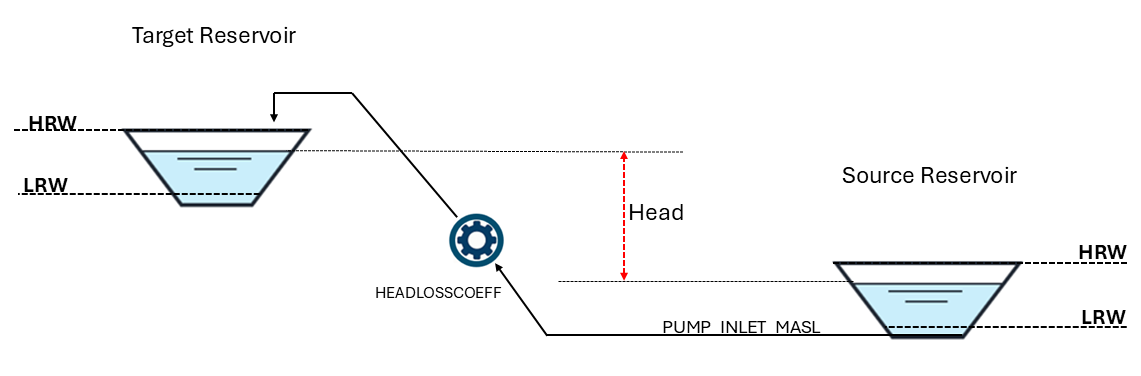
\includegraphics[width=1\linewidth]{figures/PUMP.png}
        \caption{Node type \texttt{PUMP}. Illustration of the connection of the pump between its source and target reservoirs.}
        \label{fig:pump}
    \end{figure}

    In the simulation of each time step, while the movement of water flow from the most upstream node to the most downstream node (\texttt{IDNR} 0 to \texttt{IDNR} $(N-1)$), the pump moves water from its source to the target reservoir when the simulation reaches the pumps \texttt{IDNR}. When all movement of water is simulated within each time step, the power and cost of electricity are calculated based on average head between target and source reservoirs, before the next time step is simulated.
    
	\subsubsection{Hydraulic Head and Power Calculation}

	The gross hydraulic head is computed as the average value between the target and source reservoirs within a time step, here as target minus source:

	\begin{equation}
		H_\mathrm{brutto} = \left(\frac{h_\mathrm{start}^\mathrm{tgt} + h_\mathrm{end}^\mathrm{tgt}}{2}\right) - \left(\frac{h_\mathrm{start}^\mathrm{src} + h_\mathrm{end}^\mathrm{src}}{2}\right)
        \label{eq:Pump_head}
	\end{equation}

    where $h$ are the reservoir water surface elevations denoted $_{start}$ and $_{end}$ for the beginning and end of a time step respectively, and $^{tgt}$ and $^{src}$ for target and source reservoir, respectively.
    
	Head losses are added to the head the pump must overcome, unlike Eq.~\ref{eq:Head_net} for power stations. This is done using the same quadratic formula as for poser stations and give net head as: 

	\begin{equation}
		H_\mathrm{netto} = H_\mathrm{brutto} + k \cdot Q^2
	\end{equation}
    where $k$ is the head loss coefficient (\texttt{HEADLOSSCOEF}) for the pump and $Q$ is the pumped water $\mathrm{[m^3/s]}$.

	Electrical power drawn from the grid is:

	\begin{equation}
		P = \frac{\rho g \cdot H_\mathrm{netto} \cdot Q}{\eta_\mathrm{pump}(Q) \cdot \eta_\mathrm{motor}} \quad \text{[MW]}
	\end{equation}

	where $\eta_\mathrm{pump}(Q)$ is read from a \texttt{PUMP\_CURVE}/\texttt{UNIFORM\_NORMALIZED\_CURVE} (same format as the turbine efficiency curve, Section~\ref{subsec:powerstation}) and $\eta_\mathrm{motor}$ is \texttt{STATIC\_MOTOR\_EFFICIENCY}.

	\subsubsection{Topology File Syntax}

	\begin{verbatim}
    NODE PUMP <idnr> <nodename>
    PUMP_SOURCE_IDNR <idnr>
    PUMP_TARGET_IDNR <idnr>
    PUMP_INLET_MASL <masl>
    MAX_DISCHARGE <m3/s>
    HEADLOSSCOEF <k>
    STATIC_MOTOR_EFFICIENCY <0-1>
    PUMP_STARTSTOP <value>
    UNIFORM_NORMALIZED_CURVE 11
    0.0     <0-100>
    ...
    1.0     <0-100>
    ENDNODE
	\end{verbatim}

    \subsubsection{Start and Stop Costs}
    A start/stop cost (\texttt{PUMP\_STARTSTOP}) [EUR] is incurred each time the pump
    transitions between the off state ($a = 0$) and the on state ($a > 0$), or vice versa,
    exactly as for a power station (Section~\ref{subsec:powerstation}). The cost is split
    equally between the start event and the stop event, so each transition contributes
    $\texttt{PUMP\_STARTSTOP} / 2$ to the total cost.

	\subsubsection{Numbering Requirement}
	Both \texttt{PUMP\_SOURCE\_IDNR} and \texttt{PUMP\_TARGET\_IDNR} must be higher than the pump's own \texttt{IDNR} since the pumped water is moved before either reservoir each time step.

    \begin{figure}[h!]
        \centering
        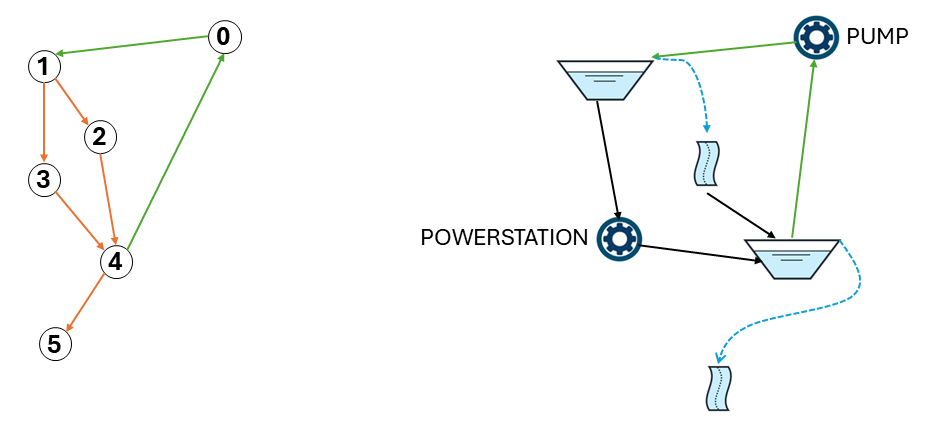
\includegraphics[width=1\linewidth]{figures/PUMP_System.png}
        \caption{Schematic of the \texttt{Mini\_pump\_test} system, and how the nodes are connected in the topology. \texttt{IDNR} 0 is the pump, and \texttt{IDNR} 3 is the power station. This illustrates how a pump can move water without following the normal rule of water flow from a node with a lower to a higher \texttt{IDNR}, but may move water between tow nodes with \texttt{IDNR} higher than itself.}
        \label{fig:Pump_system}
    \end{figure}

    \newpage
	\section{Input}
	This section describes in more detail the input files required to run HERSS. To some extent it is a repetition of what was said in earlier chapters. Feel free to skip it or have quick look \smiley{}. An efficient way to learn about the input files and their format is to just open the testdata and use it as a starting point in your own project. 
	
	\subsection{The Global Configuration File}
	\label{sec:globalconfig}

	The global configuration file is the single entry point to HERSS. It is passed as a
	command-line argument when the model is executed: \cmd{herss.exe global.txt}. 
	The file collects all top-level settings in one place: the system name, 
	paths to input and output directories, names of all other input and 
	output files, and a small number of run-time flags. 
	Lines beginning with \texttt{\#} are treated as comments and ignored.

	Table~\ref{tab:globalconfig} describes each keyword.

	\begin{table}[h]
	\centering
	\caption{Keywords in the global configuration file.}
	\label{tab:globalconfig}
	\begin{tabular}{lp{9cm}}
		\hline
		\textbf{Keyword} & \textbf{Description} \\
		\hline
		\texttt{SYSTEMNAME}         & Name of riversystem. Used in output filenames. \\
		\texttt{INPUTDIR}           & Path to the directory containing all input files. \\
		\texttt{TOPOLOGYFILE}       & Name of the topology file \\
		\texttt{INFLOWFILE}         & Name of the inflow time series file. \\
		\texttt{PRICEFILE}          & Name of the electricity price file. Also defines the simulation period and time step. \\
		\texttt{ACTIONFILE}         & Name of the file containing release and production actions. \\
		\texttt{STARTSTATEFILE}     & Name of the state file defining initial conditions (reservoir levels, channel storage). \\
		\texttt{OUTPUTDIR}          & Path to the directory where all output files are written. \\
		\texttt{OUTSTATEFILE}       & Name of the output state file written at the end of the simulation. \\
		\texttt{WRITE\_NODEFILES}   & Write individual node output files (1 = yes, 0 = no). \\
		\texttt{PRINT\_GLOBAL\_INFO}   & Print global system information to screen (\texttt{TRUE}/\texttt{FALSE}). \\
		\texttt{PRINT\_ECONOMIC\_INFO} & Print economic summary to screen (\texttt{TRUE}/\texttt{FALSE}). \\
		\hline
	\end{tabular}
	\end{table}

	\subsection{The Topology File}
	\label{sec:topologyfile}
	The topology file defines the physical structure of the river system: which nodes exist,
	what type they are, how they are connected, and all their physical parameters. It is the largest and most detailed of the input files.

	\subsubsection{File Structure}

	The file consists of a sequence of node blocks. Each block opens with a \texttt{NODE}
	declaration and closes with \texttt{ENDNODE}. Lines beginning with \texttt{\#} are
	comments. The general structure of a node block is:

	\begin{verbatim}
	NODE  <NODETYPE>  <IDNR>  <NAME>
	<keyword>  <value>
	...
	ENDNODE
	\end{verbatim}

	where \texttt{NODETYPE} is one of \texttt{RESERVOIR}, \texttt{PSTATION}, \texttt{PUMP}, or
	\texttt{CHANNEL}, \texttt{IDNR} is the unique integer node identifier, and \texttt{NAME}
	is a descriptive label used in output files and log messages.

	As described in Section \ref{sec:topo_start}, node identifiers must be assigned in
	strict upstream-to-downstream order. HERSS simulates nodes in ascending order of
	\texttt{IDNR} at each time step, so all upstream nodes must have lower identifiers than the nodes they drain into.

	Downstream connections are specified differently for each node type:

	\begin{itemize}
	\item \texttt{RESERVOIR}: downstream connections are implicit in the outlet
	keywords (\texttt{OUTLET\_TUNNEL}, \texttt{OVERFLOW\_CURVE},
	\texttt{OUTLET\_HATCH}, \texttt{OUTLET\_AUTO\_QMIN}), each of which
	carries a downstream \texttt{IDNR}.
	\item \texttt{PSTATION}: the downstream node is specified with
	\texttt{DOWNLINK\_IDNR}.
	\item \texttt{CHANNEL}: the downstream node \texttt{IDNR} is given on the
	\texttt{NODE} line itself. A value of \texttt{-9} indicates no downstream
	connection, i.e.\ the system outlet.
    \item \texttt{PUMP}: This node only specifies which nodes water is moved between with two nodes of higher \texttt{IDNR} than itself by specifying \texttt{PUMP\_SOURCE\_IDNR} and \texttt{PUMP\_TARGET\_IDNR}.
	\end{itemize}


	The parameters within each node block are described in detail in section \ref{sec:nodetypes}.

	The topology file is used to specify all the nodes that the riversystem consists of. Each node needs an identification number (idnr). The first node needs the idnr to be zero (0), and the following nodes increasing. Upstream and downstream nodes also needs to be specified. The lowest outlet node (ocean or most downstream part of riversystem is identifies if the downstream node is set to -9). The topology file is typically 
	made by looking at maps/GIS description of your system. 



	\subsection{The Price file}
	\label{sec:pricefile}

	The price file supplies the electricity spot price time series and the end-of-horizon
	water value used to evaluate remaining storage. It is the file that also defines the
	simulation period and the number of time steps: HERSS counts the data rows in the price
	file during initialisation to determine the total number of time steps (\texttt{stps}).
	All other time series files (inflow, actions) must contain the same number of rows.

	\subsubsection{File Format}

	The file has a fixed two-line header followed by one data row per time step:

	\begin{verbatim}
	RESTPRICE   <value>
	Date        Price
	<timestamp> <price>
	<timestamp> <price>
	...
	\end{verbatim}

	\begin{description}
	\item[\texttt{RESTPRICE}] The water value, or rest price, at the end of the
	planning horizon [currency/MWh]. This value is used to estimate the economic
	worth of water remaining in the reservoirs at the end of the simulation.
	It must appear on the first non-comment line.
	
	\item[\texttt{Date Price}] A fixed column header line. Must appear as the second
	non-comment line.
	
	\item[Timestamp] Each data row begins with a timestamp in one of the formats
	supported by HERSS: \texttt{yyyymmddhh}, \texttt{yyyymmdd}, \texttt{yyyy-mm-dd},
	or \texttt{yyyy-mm-dd-hh}. The time step $\Delta t$ is derived automatically
	from the difference between consecutive timestamps, enabling variable temporal
	resolution within the same file (see also section \ref{sec:multitemp} ).
	
	\item[Price] The electricity spot price for the time step [currency/MWh]. HERSS is
	currency-agnostic; any consistent currency unit may be used. The test dataset
	uses EUR/MWh.
	\end{description}

	It is assumed that the entire river system lies within a single price area, so one price
	series applies uniformly to all power stations and penalty calculations.

	\subsection{The Inflow file}
	\label{sec:inflowfile}

	The inflow file provides the lateral inflow time series for each reservoir in the river system. Inflow represents natural runoff entering the river network at a specific location, for	example precipitation-driven runoff from a catchment draining directly into a reservoir.
	Inflows are given in [m$^3$/s] and are provided for each simulation time step.

	\subsubsection{File Format}
	The file has a single header line followed by one data row per time step. The header
	identifies the columns by their reservoir node \texttt{IDNR}:

	\begin{verbatim}
	Date_NodeID  <res_idnr_0>  <res_idnr_1>  ...
	<timestamp>  <Q_0>     <Q_1>     ...
	<timestamp>  <Q_0>     <Q_1>     ...
	...
	\end{verbatim}

	The keyword \texttt{Date\_NodeID} is mandatory and must appear as the first token
	on the header line. After the keyword, the remaining tokens on the same line are
	the integer node identifiers (\texttt{IDNR}) for the reservoirs in the system. 
	The first column of each data row is a timestamp in one of the
	formats accepted by HERSS (\texttt{yyyymmddhh}, \texttt{yyyymmdd},
	\texttt{yyyy-mm-dd}, or \texttt{yyyy-mm-dd-hh}). The timestamps must match
	exactly the timestamps in the price file. HERSS validates each row and will
	report an error on any date mismatch.
	
	Each of the remaining column gives the inflow [m$^3$/s] entering the
	node whose \texttt{IDNR} was listed in the corresponding header position.
	The number of data rows must equal the number of time steps defined by the price file.

	For a larger system with inflow entering multiple reservoir nodes, the header and data rows would contain multiple columns, for example:

	\begin{verbatim}
	Date_NodeID  0     3     7
	2026050700   1.50  0.80  2.10
	2026050701   1.35  0.75  1.95
	...
	\end{verbatim}

	Here nodes~0, 3, and~7 each receive their own inflow series. All other nodes in the system
	receive zero lateral inflow by default.


	
	\subsection{The Actions File}
	\label{sec:actionsfile}

	The actions file specifies how each controllable element in the river system is operated
	at every time step. An action is a dimensionless control signal with values in the range
	$[0.0,\, 1.0]$, where $0.0$ means the element is fully closed or off and $1.0$ means
	it operates at its maximum capacity. Intermediate values represent partial operation.

	Actions are defined for the following controllable elements:

	\begin{itemize}
	\item \textbf{Power station generators}: the action sets the discharge through the
	turbine as a fraction of the generator's maximum discharge - \\ 
	(\texttt{GENERATOR\_MAX\_DISCHARGE}). Each generator in a multi-generator station
	has its own action column.
	\item \textbf{Reservoir hatches} (\texttt{OUTLET\_HATCH}): the action controls the
	gate opening, scaling the discharge linearly between the defined minimum and
	maximum hatch flows.
    \item \textbf{Pumps}: the action sets the discharge through the
	pump as a fraction of the pumps maximum discharge (\texttt{MAX\_DISCHARGE}).
	\end{itemize}

	\subsubsection{File Format}

	The format mirrors the inflow file: a single header line followed by one data row per
	time step.

	\begin{verbatim}
	Date_NodeID  <node_gen>  <node_gen>  ...
	<timestamp>  <action>    <action>    ...
	<timestamp>  <action>    <action>    ...
	...
	\end{verbatim}


	\begin{description}
	\item[\texttt{Date\_NodeID}] Mandatory keyword on the header line. The remaining
	tokens on the header line identify each column using the notation
	\texttt{<idnr>\_<generator\_index>}, where \texttt{idnr} is the node identifier
	and \texttt{generator\_index} is the zero-based generator number within that
	node. For example, \texttt{5\_0} refers to generator~0 of the power station at
	node~5, and \texttt{5\_1} refers to its second generator.
	
	\item[Timestamp] First column of each data row. Must use one of the HERSS date
	formats (\texttt{yyyymmddhh}, \texttt{yyyymmdd}, \texttt{yyyy-mm-dd}, or
	\texttt{yyyy-mm-dd-hh}) and must match the timestamps in the price file exactly.
	HERSS validates each row and reports an error on any mismatch.
	
	\item[Action values] Each remaining column gives the action $a \in [0.0,\, 1.0]$
	for the element identified in the header. The number of data rows must equal
	the number of time steps defined by the price file.
	\end{description}

	\subsubsection{Example}

	In the mini uTAHPS example, only node~1 (\texttt{SVOLETJONN}) has one generator, so the
	actions file has a single data column:

	\begin{verbatim}
	Date_NodeID  1_0
	2026050700   0.66
	2026050701   0.00
	2026050702   0.00
	2026050703   0.00
	2026050704   1.00
	...
	\end{verbatim}

	For a system with multiple power stations and generators, the header lists all controllable
	elements and the data rows supply each action independently:

	\begin{verbatim}
	Date_NodeID  1     5_0   5_1
	2026050700   0.00  0.80  0.70
	2026050701   0.70  0.75  0.00
	...
	\end{verbatim}

	Here node~1 is a reservoir with the hatch outlet in operation (no underscore). Node 5 is a powerstation with two generators operating independently. Only elements that have a corresponding action column are controlled; all other nodes receive no action signal and behave according to their passive or automatic settings.

	
	\subsection{The State File}
	\label{sec:statefile}
	
	The state file defines the initial hydraulic condition of the river system at the start of
	the simulation. It is the mechanism that connects successive simulation runs: the output
	state file written at the end of one run (\texttt{OUTSTATEFILE}) can be used directly as
	the input state file (\texttt{STARTSTATEFILE}) for the next run, enabling seamless
	chaining over a long planning horizon.
	
	\subsubsection{File Format}
	
	The file contains one line per node that carries state. Lines beginning with \texttt{\#}
	are comments and are ignored. Each node line follows the pattern:
	
	\begin{verbatim}
		NODE  <NODETYPE>  <IDNR>  <NAME>  <value(s)>
	\end{verbatim}
	
	Different node types each have their own format:
	
	\begin{description}
		\item[\texttt{NODE RESERVOIR \textnormal{\textit{idnr name fr}}}]
		The reservoir initial condition is given as a \emph{filling fraction}
		$f_r \in [0.0,\, 1.0]$, where $0.0$ corresponds to the Lowest Regulated Water
		level (LRW) and $1.0$ corresponds to the Highest Regulated Water level (HRW).
		Values outside this range are physically possible (the reservoir may be below LRW
		or spilling above HRW) and are accepted by HERSS. The initial stored volume is
		computed as:
		\[
		V_\mathrm{start} = V_\mathrm{LRW} + f_r \cdot (V_\mathrm{HRW} - V_\mathrm{LRW})
		\]
		
		\item[\texttt{NODE PSTATION \textnormal{\textit{idnr name P}}}]
		The power station initial condition is the production [MWh] at the last time step
		of the previous run. This value is used to evaluate start/stop cost transitions
		at the first time step of the new simulation. A value of \texttt{0.0} means the
		station was off at the end of the previous period.
		
		\item[\texttt{NODE CHANNEL \textnormal{\textit{idnr name $S_0$ $S_1$ \ldots $S_{N-1}$}}}]
		The channel initial condition is the water volume stored in each of the $N$
		cascaded linear reservoirs [Mm$^3$]. The number of values must exactly match
		\texttt{N\_CASCADE\_LINRES} as defined for this node in the topology file.
		These values initialise the routing model so that the channel carries the correct
		amount of in-transit water from the start.

        \item[\texttt{NODE PUMP \textnormal{\textit{idnr name P}}}] The PHS facility's initial condition is the energy consumed [MWh] at the last time step
		of the previous run, written as a positive value. This value is used to evaluate start/stop cost transitions
		at the first time step of the new simulation. A value of \texttt{0.0} means the pump was off at the end of the previous period.  
	\end{description}
	
	\subsubsection{Example}
	
	The mini uTAHPS state file \file{start\_state.txt}:
	
	\begin{verbatim}
		# STATEFILE MINI UTAHPS
		
		# NODE RESERVOIR IDNR NAME RES_FR
		NODE RESERVOIR 0 HJELLE 0.67
		
		# NODE PSTATION IDNR NAME MWh
		NODE PSTATION 1 SVOLETJONN 0.0
		
		# NODE CHANNEL IDNR NAME LINRES1_Mm3 LINRES2_Mm3 LINRES3_Mm3
		NODE CHANNEL 2 VANAROSEN 0.001 0.002 0.003
	\end{verbatim}
	
	Here the \texttt{HJELLE} reservoir starts at 67\,\% of its active storage range, the
	power station \texttt{SVOLETJONN} was off at the end of the previous period, and the
	\texttt{VANAROSEN} channel carries three small water volumes corresponding to its three
	cascaded linear reservoirs.



	\section{Output Files}
	\label{sec:output}

	After a simulation has finished, HERSS writes a set of plain-text output files to the
	directory specified by \texttt{OUTPUTDIR} in the global configuration file. For a system
	named \texttt{mini\_uTAHPS\_hourly}, the output folder will contain the following files:

	\begin{itemize}
	\item \file{node0\_HJELLE.txt}, \file{node1\_SVOLETJONN.txt}, \file{node2\_VANAROSEN.txt} --- individual node output files (written only if \texttt{WRITE\_NODEFILES 1})
	\item \file{reservoirs\_mini\_uTAHPS\_hourly\_out.txt} --- reservoir filling fractions for all reservoirs
	\item \file{riversystem\_mini\_uTAHPS\_hourly\_output.txt} --- aggregated river system summary
	\item \file{outstate.txt} --- end state of the simulation
	\end{itemize}

	The exact filenames depend on the system name (\texttt{SYSTEMNAME}) and the output state
	filename (\texttt{OUTSTATEFILE}) set in the global configuration file.

	\subsection{Node Output Files}

	When \texttt{WRITE\_NODEFILES} is set to \texttt{1}, HERSS writes one output file per node,
	named \file{node\textit{idnr}\_\textit{NODENAME}.txt}. These files contain the most
	detailed simulation results and are the primary source for time series plots.

	Each file begins with a short header identifying the node type and name, followed by a
	time series with one row per time step. The columns depend on the node type and are
	described in Section~\ref{sec:nodetypes}. Typical variables include inflow,
	reservoir water level, reservoir filling fraction, tunnel and hatch discharge, overflow,
	power production, hydraulic head, income, and cost.

	\subsection{Reservoir Filling Fractions File}

	The file \file{reservoirs\_\textit{systemname}\_out.txt} contains the time series of
	filling fractions for every reservoir in the system, with one column per reservoir. An
	example from the mini uTAHPS system:

	\begin{verbatim}
	Riversystem mini_uTAHPS_hourly reservoir fractions [fr]
	YYYY MM DD HH HJELLE
	2026 5 7 0 0.6695
	2026 5 7 1 0.6701
	...
	\end{verbatim}

	This file is particularly convenient for plotting reservoir levels and checking storage
	trends across the simulation period.

	\subsection{River System Summary File}

	The file \file{riversystem\_\textit{systemname}\_output.txt} provides a compact summary of
	the entire simulation. It contains:

	\begin{itemize}
	\item A node inventory listing each node, its type, and its remaining water volume
	[Mm$^3$] at the end of the simulation.
	\item A global water balance: starting volume, total inflow, total outflow, and ending
	volume, with a check that the balance closes to zero.
	\item Aggregated economic results, including total production [MWh], total income,
	total costs (LRW penalty, start/stop costs, minimum flow violations), total profit,
	the estimated value of remaining water, and the final value function.
	\end{itemize}

	The value function is the quantity typically used by optimisation algorithms to evaluate
	the quality of an action sequence:

	$$
	V = \text{tot\_profit\_Euro} + \text{tot\_remaining\_Euro}
	$$
	
	\subsubsection{Output State File}
	At the end of every simulation, HERSS writes an output state file (named by
	\texttt{OUTSTATEFILE} in the global configuration). The format is identical to the input
	state file described above. For reservoirs, the written value is the simulated filling
	fraction $f_r$ at the final time step. For power stations it is the final production
	value. For channels it is the volume held in each cascaded linear reservoir at the end of
	the last time step. This file can immediately be used as \texttt{STARTSTATEFILE} for a
	subsequent run.

	\section{Multi-Temporal Resolution and date formats}
	\label{sec:multitemp}

	Multi-temporal resolution is introduced in order to reduce computational 
	burden in long simulation horizons while retaining sufficient process realism. 
	When the full simulation period is represented at a uniformly fine timestep, such as hourly resolution, the number of timesteps becomes large and model runtime increases substantially. This is especially important in applications involving repeated simulations. This could be optimization, scenario analysis, or stochastic sampling.
	
	
	\begin{table}[h]
	\centering
	\caption{Example of variable temporal resolution input. The time step $\Delta t$ is
		derived internally from the difference between consecutive timestamps.}
	\label{tab:variable_dt}
	\begin{tabular}{lrrr}
		\hline
		\textbf{Datetime} & \textbf{Price} & $\boldsymbol{\Delta t}$ \textbf{[s]} & \textbf{Resolution} \\
		\hline
		2024010100 & 45.2 & 3\,600  & hourly \\
		2024010101 & 43.8 & 3\,600  & hourly \\
		2024010102 & 41.1 & 3\,600  & hourly \\
		2024010103 & 39.5 & 3\,600  & hourly \\
		...  & ... & ...  & ... \\
		\hline
		2024010200 & 52.3 & 86\,400 & daily  \\
		2024010300 & 55.1 & 86\,400 & daily  \\
		2024010400 & 50.7 & 86\,400 & daily  \\
		...  & ... & ...  & ... \\
		\hline
		2024010800 & 48.0 & 604\,800 & weekly \\
		2024011500 & 46.5 & 604\,800 & weekly \\
		2024012200 & 44.2 & 604\,800 & weekly \\
		\hline
	\end{tabular}
	\end{table}
	
	In addition, the required temporal detail is not constant across all parts of the simulation horizon. 
	Short-term operational processes may require fine temporal resolution, whereas long-term planning, seasonal storage dynamics, and economic evaluation may be represented adequately at daily or weekly resolution. 
	A variable-resolution framework therefore allows computational effort to be allocated where it is most informative.

	The use of multiple temporal resolutions is also justified by the fact that input data often have different effective information content over time. High-frequency forcing may be important during rapid hydrological events or short-term market fluctuations, while lower-frequency representation may be sufficient during slowly varying periods. 
	Accordingly, a multi-temporal routing formulation provides a practical compromise between computational efficiency and process representation.

	The main methodological requirement is that the routing model must remain mass-conserving and numerically consistent when the timestep changes. This is necessary to ensure that coarser temporal resolution reduces computational cost without introducing unacceptable distortion of storage dynamics, attenuation, or delay. Table \ref{tab:variable_dt} shows how variable timestep length can be used in the input files. In the last timestep we assume $\Delta t$ is the same as in the preceding step. 
	
		

	%--------------------------------------------------------------------------------
	%--------------------------------------------------------------------------------
	%--------------------------------------------------------------------------------
	\chapter{Tutorial and feature guide}
	This chapter provides a tutorial and presentation of several test datasets designed to explore various functionality in the HERSS model. 
	
	\section{Testdata Reservoir Cascade A}
	We will now explore the test dataset provided in the folder: \folder{./res\_casc\_A/}.
	The node structure and the topology of this dataset is illustrated in Figure \ref{fig:rescasc1}. 
	The system has two reservoirs, one powerstation and three channels. There are two features that we will explore in this example: hatch release directly from a reservoir, and the use of multi generators at a powerstation. We also use daily simulation steps.
	
	\begin{figure}[h]
	\centering
	\includegraphics[width=0.85\textwidth]{./figures/res_casc1.pdf}
	\caption{Node structure and topology of the reservoir cascade test dataset}
	\label{fig:rescasc1}
	\end{figure}

	\newpage
	
	Now let's open the \file{actions.txt} inputfile. You should see the following: 
	
	\begin{verbatim}
		Date_NodeID 0 4_0 4_1
		20220901 0.7 0.8 0.8
		20220902 0.8 0.8 0.0
		20220903 0.9 0.8 0.0
		...
	\end{verbatim}
	
	In the first row of the actions file, you can see four columns. The first column is the date, and in the next three we have actions. The action for this system consist of the hatch release from reservoir RES\_A, which is in node 0. This corresponds to column two. The last two columns are the action for generator 0 and 1, in the powerstation named PSTAT\_B, in node 4. Note the name convention. \\
	
	In the topology file, at line 29 and 30, you will see the flags setting usage of hatch outflow from reservoir RES\_A (node 0). We can see that the maximum outflow from the hatch is set to 6.0 m$^3$/s. 
	
	\begin{verbatim}
	# OUTLET_HATCH downstream_nodeid, qmin_hatch, qmax_hatch, hatch_masl
	OUTLET_HATCH 1 0.0 6.0 848.0
	\end{verbatim}


	
	Run herss for this system with the command \cmd{../../herss.exe global.txt}. \\
	
	Inside the folder \folder{./res\_casc\_A/output/} you will see all the different output files generated by HERSS. Now let's take a look at the simulation results for reservoir RES\_A (node 0). Figure \ref{fig:res_a} shows the inflow to the reservoir in (a), the hatch outflow and overflow in (b), and the reservoir filling in percent in (c). The maximum hatch outflow was set to 6.0 m$^3$/s in the topology file. This means that actions with values of 1.0 will release maximum hatch flow (6.0 m$^3$/s). We can see that in Figure \ref{fig:res_a} (b), the hatch outflow is never above this level. We can also see that the reservoir is above full in two time periods. Overflow is then activated and we see that overflow is larger than zero.
	
	\newpage 

	\begin{figure}[h]
	\centering
	\includegraphics[width=0.85\textwidth]{./figures/res_a.pdf}
	\caption{Simulation results for the reservoir RES\_A (node 0)}
	\label{fig:res_a}
	\end{figure}

	Figure \ref{fig:pstat_a} shows the simulation results for the powerstation PSTAT\_B (node 4), and the connected reservoir, RES\_B. The figure has four subplots. In subplot (a), we see the inflow to the upstream reservoir. In (b) the reservoir filling is plotted. The actions for generator 0 and 1 are illustrated in subplot (C). In the lowest subplot in Figure \ref{fig:pstat_a}, the total power is shown. In the beginning of the time period only one generator is running. This proudces around 40 MWh pr day. Later in the time period, around 22-26 Sep, both generators are running at fairly high actions. The system then produces around 75 MWh pr day. This illustrates the usage of more than one generator in a single powerstation. 
	
	\clearpage
	\begin{figure}[h]
		\centering
		\includegraphics[width=0.95\textwidth]{./figures/pstat_res_casc.pdf}
		\caption{Simulation results for the powerstation PSTAT\_B (node 4), and the connected reservoir RES\_B (node 4)}
		\label{fig:pstat_a}
	\end{figure}
	
	\clearpage 



	\section{Running HERSS from Python}
	\label{sec:python}

	\subsection{What is cppyy?}

	\texttt{cppyy} is an automatic Python-C++ bindings library that allows Python code
	to call C++ classes, functions, and variables directly at runtime, without writing
	any wrapper code. Under the hood, \texttt{cppyy} runs a small C++ interpreter that reads your header files and figures out what classes, functions, and variables exist in your C++ code. It then automatically makes those available as Python objects --- so you can call a C++ function from Python just as if it were a regular Python function, without ever writing any glue code yourself.
	
	
	The key advantage of \texttt{cppyy} is that no binding code needs to be written or compiled.
	You load a shared library and include the corresponding header file, and all
	classes and functions declared in that header become immediately available as
	Python objects. \\

	Install \texttt{cppyy} with:
	\begin{verbatim}
		pip install cppyy
	\end{verbatim}

	\noindent This is where the HERSS shared library file (\file{herss.so}) comes in handy. It is part of the HERSS source code and is made ready during compilation of HERSS. 
	
	

	% ---------------------------------------------------------------
	\subsection{Loading HERSS into Python}

	The two lines below are all that is needed to make the entire HERSS C++ API
	available in Python:

	\begin{verbatim}
	import cppyy
	cppyy.load_library("../src/herss.so")
	cppyy.include("../src/herss.h")
	\end{verbatim}

	After these calls, all classes declared in \texttt{herss.h} --- including
	\texttt{GlobalConfig}, \texttt{Dataset}, \texttt{Herss}, \texttt{Logger}, and
	others --- are accessible through the \texttt{cppyy.gbl} namespace.

	% ---------------------------------------------------------------
	\subsection{Initialising the Logger}

	HERSS uses an internal logging system. When running from Python, the
	\texttt{main()} function is never called, so the logger must be initialised
	manually before any other HERSS code is executed:

	\begin{verbatim}
	version      = cppyy.gbl.VERSION
	version_date = cppyy.gbl.VERSION_DATE
	logfilename  = f"herss_{version}_{version_date}.log"
	
	if not cppyy.gbl.Logger.instance().init(logfilename):
	print(f"Could not open log file: {logfilename}")
	\end{verbatim}

	\noindent All subsequent \texttt{LOG\_WARN}, \texttt{LOG\_ERR}, and
	\texttt{LOG\_MSG} calls inside C++ will write to this file.

	% ---------------------------------------------------------------
	\subsection{Setting Up a Simulation}

	A HERSS simulation is set up in the same sequence as the C++ \texttt{main()}
	function. The following steps must be performed in order.

	\paragraph{1. Create and configure GlobalConfig.}
	\begin{verbatim}
	gc = cppyy.gbl.GlobalConfig()
	gc.globalfile = "../data/mini_utahps_daily/global.txt"
	gc.readGlobalFile()
	gc.inputdir  = "../data/mini_utahps_daily/"
	gc.outputdir = "../data/mini_utahps_daily/output/"
	gc.SetDirectoriesAndFilenames()
	gc.Diagnose()
	gc.checkNrSteps()
	\end{verbatim}

	\paragraph{2. Read input data.}
	\begin{verbatim}
		data = cppyy.gbl.Dataset(gc)
		data.readAllData()
	\end{verbatim}

	\paragraph{3. Create the Herss object and prepare the simulation.}
	\begin{verbatim}
	herss = cppyy.gbl.Herss(gc)
	herss.prepaireSimulation(data)
	herss.rs.DiagnoseRiversystemConfiguration()
	\end{verbatim}

	\paragraph{4. Run the simulation.}
	\begin{verbatim}
	herss.Simulate()
	vf = herss.rs.CalcVF(data.restprice)
	print("Value function =", vf)
	\end{verbatim}

	% ---------------------------------------------------------------
	\subsection{Reading and Writing Simulation State}

	After \texttt{Simulate()} has been called, results can be read back through
	the \texttt{Herss} interface methods. Table~\ref{tab:herss_api} lists the
	most commonly used functions.

	\begin{table}[h]
	\centering
	\begin{tabular}{ll}
		\hline
		\textbf{Method} & \textbf{Description} \\
		\hline
		\texttt{GetPrice(t)} & Electricity price at timestep $t$ \\
		\texttt{GetInflowInNode(t, node)} & Local inflow at node at timestep $t$ [m$^3$/s] \\
		\texttt{GetReservoir\_Init\_fr(idnr)} & Initial reservoir filling fraction \\
		\texttt{GetReservoirLevel\_fr(node, t)} & Reservoir filling fraction at end of timestep $t$ \\
		\texttt{GetAction(node, gen, t)} & Action for generator \texttt{gen} at node at timestep $t$ \\
		\hline
		\texttt{SetPrice(t, price, restprice)} & Override price and rest price at timestep $t$ \\
		\texttt{SetInflowInNode(t, node, q)} & Override inflow [m$^3$/s] at node at timestep $t$ \\
		\texttt{SetReservoir\_Init\_fr(node, fr)} & Override initial reservoir filling fraction \\
		\texttt{SetAction(node, gen, t, value)} & Set action for generator \texttt{gen} at timestep $t$ \\
		\hline
	\end{tabular}
	\caption{Commonly used \texttt{Herss} interface methods available from Python.}
	\label{tab:herss_api}
	\end{table}

	After modifying prices, inflows, or actions, call \texttt{herss.Simulate()}
	again. It is not necessary to call \texttt{prepaireSimulation()} again;
	\texttt{Simulate()} reinitialises reservoir states internally on every call.

	% ---------------------------------------------------------------
	\subsection{The pyherss.py Example Script}

	A complete working example is provided in \texttt{py\_src/pyherss.py}.
	This script demonstrates the full workflow described above, including reading
	results, overriding inputs, and re-running the simulation.

	New users are encouraged to work through the script one block at a time
	in an interactive Python session (e.g.\ using Jupyter or IPython):

	\begin{enumerate}
		\item Run only the \texttt{cppyy} load and include lines. Verify that
		no import errors occur.
		\item Create \texttt{gc} and call \texttt{readGlobalFile()}. Print
		\texttt{gc.nr\_nodes} and \texttt{gc.stps} to confirm the
		configuration was read correctly.
		\item Create \texttt{data} and call \texttt{readAllData()}. Print
		\texttt{data.price[0]} to verify that price data is loaded.
		\item Create \texttt{herss}, call \texttt{prepaireSimulation(data)},
		then \texttt{Simulate()}. Print the value function.
		\item Experiment with \texttt{SetPrice()}, \texttt{SetInflowInNode()},
		and \texttt{SetAction()}, then call \texttt{Simulate()} again and
		observe how the value function changes.
	\end{enumerate}

	\noindent This incremental approach makes it easy to isolate the source of
	any error, since each step depends only on the steps before it.

	\begin{quote}
		\textit{Note:} \texttt{cppyy} translates C++ errors and \texttt{LOG\_ERR}
		calls into Python exceptions. If a call terminates unexpectedly, check both
		the Python traceback and the HERSS log file for details.
	\end{quote}

	%-----------------------------------------------------------------------------------------
	%-----------------------------------------------------------------------------------------
	%-----------------------------------------------------------------------------------------
	\chapter{Datasets}
	This chapter present test datasets that are part of the HERSS repository.
	
	\section{Upper Tovdalen Artificial Hydro Power System (uTAHPS)}
	
	\subsection{Riversystem}
	In this open source project, we have defined an artificial hydropower system that doesn’t exist in
	the real world. We have synthetically placed a hydropower system in the upper part of the
	Tovdalen river system, located in southern Norway. We define this system as the Upper Tovdalen
	Artificial Hydro Power System (uTAHPS). The system consists of four reservoirs and four
	powerstations with varying nr of generators and penstock configuration. A schematic map of the
	system is illustrated in Figure \ref{fig:utahps_river}. Red dots are powerstations, the blue regions are illustrations of the synthetic reservoirs. 
	The drainage area for each reservoir is also noted in the figure. 
	
	Figure \ref{fig:utahps_names} shows the uTAHPS riversystem with node numbers and names, and their connections. This node-network is defined in the topology files that the HERSS
	model reads. Note that the uTAHPS can be modelled with fewer nodes depending on the usecase. In chapter \ref{chap:starting} we used the uppermost three nodes of this system as an example. 

	\clearpage
	
	\begin{figure}[h]
		\centering
		\includegraphics[width=0.9\textwidth]{./figures/utahps_river.png}
		\caption{Map of Upper Tovdalen Artificial Hydro Power System}
		\label{fig:utahps_river}
	\end{figure}
	
	\begin{figure}[h]
		\centering
		\includegraphics[width=0.9\textwidth]{./figures/utahps_names.pdf}
		\caption{Topology of the uTAHPS. Node number and names included.}
		\label{fig:utahps_names}
	\end{figure}
	\clearpage

	\subsection{Timeseries}
	In addition to riversystem description for the uTAHPS a set of timeseries are also provided. 
	Hourly, daily, and a multi-temporal dataset of inflow and price are provided. The selected time period goes from 1 Sep,2022 until 31 Aug, 2023.
	
	\subsubsection{Inflow}
	In the uTAHPS system it is assumed that the four reservoirs receive local inflow. 
	The timeseries for these reservoirs are generated from observed streamflow data 
	extracted from the Sildre open database available from The Norwegian Water 
	Resources and Energy Directorate (www.nve.no, https://sildre.nve.no/). 

	The inflow time series for the four reservoirs (HJELLE, GRESSE, TOPSY, and KROKNESVATN) were derived from observed streamflow recorded at two nearby hydrological gauging stations, Austenå and Songedalsåi. Local inflow to each reservoir was estimated by scaling the observed streamflow by catchment area, with manually adjusted weights applied to account for differences in catchment characteristics. This approach is a pragmatic method when direct observations at the reservoir inlets are not available. Figure \ref{fig:utahps_inflow} shows the timeseries of inflow to each of the four reservoirs in uTAHPS. 
	
	\begin{figure}[h]
		\centering
		\includegraphics[width=0.95\textwidth]{./figures/utahps_inflow.pdf}
		\caption{Timeseries plot of the inflow to four reservoirs in uTAHPS}
		\label{fig:utahps_inflow}
	\end{figure}
	
	\subsubsection{Energy price}
	The uTAHPS system is located in the NO2 price region in Norway. Historical data for this region is
	available through Forbrukerrådet ( https://www.forbrukerradet.no/). These data were converted
	to Euro/MWh assuming 1 Euro = 10 NOK and Value Added Tax of 25 \%. The data can be downloaded from: \newline 
	https://www.forbrukerradet.no/strompris/spotpriser/. 
	Note that HERSS is agnostic to the currency units used. It could be NOK/MWh, Euro/MWH. 
	
	
	
	\subsubsection{Actions}
	The timeseries of actions (production) for each power station were manually set in each
	timestep.
		

	\subsubsection{uTAHPS datasets}
	There are several different datasets available for the uTAHPS. These are located under the folder \folder{./data/}. They have all been tested with the latest version of the \file{herss.exe}. Some of the datasets have also been used in previous chapters. The different datasets are designed to test different types of features. Take a look in the topology files and timeseries files to see how different features are used. 

	\vspace{1em}
	\dirtree{%
	.1 herss/.
	.2 data/.
	.3 mini\_utahps\_daily/.
	.3 mini\_utahps\_hourly/.
	.3 mini\_utahps\_spillway/.
	.3 mini\_utahps\_new\_inputformat/.
	.3 res\_casc\_A/.
	.3 res\_casc\_B/.
	.3 res\_casc\_C/.
	.3 res\_casc\_D/.
	.3 utahps\_daily/.
	.3 utahps\_hourly/.
	.3 utahps\_multires/.
	.3 utahps\_daily\_new\_format/.
	}	
	\vspace{1em}

	
	Figure \ref{fig:utahps_multires} shows a plot of the timeseries data avaiable in the \folder{./utahps\_multires/}.


	\begin{figure}[h]
	\centering
	\includegraphics[width=0.95\textwidth]{./figures/utahps_multires.pdf}
	\caption{Multi-temporal timeseries plot of electricity price}
	\label{fig:utahps_multires}
	\end{figure}


	
	%---------------------------------------------------------------------
	%---------------------------------------------------------------------
	\chapter{Known Issues and Future Work}
	\label{chap:future}
	This chapter summarizes known limitations/bugs in the current version of HERSS,
	as well as planned improvements and ideas for future development. Some features have been implemented, but due to substantial code changes, they have not been quality controlled in the new version. 
	

	\section{Known Issues}


	\subsection{Automatic Minimum Flow Release}
	The automatic minimum flow release feature for reservoirs
	(\texttt{OUTLET\_AUTO\_QMIN}) is somewhat implemented, but we need to make a small testdataset showing that it works as intended.

	\subsection{Minimum Flow Constraints in Channels (QMIN)}
	Minimum discharge requirements in channel nodes (\texttt{QMIN}) are partially
	implemented. The penalty cost structure exists in the code but the
	time-period parsing and quality control have not been completed.


	\subsection{Maximum Adjustment Penalty}
	The penalty for excessive production adjustments within a day
	(\texttt{MAX\_ADJUST}) has been implemented but has not been quality
	controlled. 


	\subsection{Generator Max Discharge}
	In the current version there are are two variables with almost the same name. These are GENERATOR\_MAX\_DISCHARGE and POWSTAT\_MAX\_DISCHARGE. Do a quality control of this, and maybe remove one of them. 


	\subsection{Start of Multi-Generator}
	Start state and end state when using multi-generators is not implemented. All generators are set to same state. 


	\section{Future Work}

	\subsection{Multi-Reservoir Water Value Calculation}
	Extending the water value calculation to multi-reservoir systems would be useful. 
	One approach is to use a gradient-based sensitivity method,
	perturbing the reservoirs individually and measuring the
	change in the value function.

	\subsection{Flood Level Penalty}
	A flood level penalty (\texttt{FLOODLEVEL\_PENALTY}) has been introduced
	in the topology file format and the corresponding variable is read, but
	the penalty is not yet applied in the simulation. This need quality control. 

	\subsection{Interface to python}
	HERSS is designed to be called from Python via \texttt{cppyy}, enabling
	integration with other frameworks. For now the python usage is linked to 
	the textfile inputs required by C++. It would be nice to be able initiate
	a new HERSS object entirely within Python. 

	\subsection{Variable Timestep Support Throughout}
	Variable timestep support has been introduced in the simulation loop
	and the water balance checks, but some parts of the codebase
	(notably the start/stop cost calculation and the adjustment cost
	calculation) still assume a fixed hourly timestep. A full audit
	and update of all timestep-dependent calculations is needed.

	\subsection{Parallel Simulation}
	For use cases with multi-scenarios (optimization), running many
	simulations in parallel would significantly reduce computation time.
	Since each \texttt{Herss} object is independent, parallelization
	at the scenario level is straightforward and could be implemented 
	either in C++ or from Python. 

	\subsection{Improved Topology File Validation}
	At present, topology file errors are caught at runtime, often deep inside
	a simulation. A dedicated validation pass before the simulation starts---
	checking that all node IDs are consistent, all downstream connections
	are valid, and all required keywords are present---would make error
	messages clearer and easier to act on. This has been partly implemented, but should be further improved. 

	\subsection{Output and Visualisation}
	The current output is written to plain text node files and a river system
	summary file. Supporting structured output formats such as NetCDF or
	CSV with consistent column naming would simplify post-processing and
	integration with tools such as GMT plotting scripts.
	
	
	\subsection{Automatic generation of node networks}
	Putting together the topology file is time consuming and complicated for larger riversystems. We need to design a method for automatic generation of topology files based on map data. 


	%-------------------------------------------------------------------------
	%-------------------------------------------------------------------------
	%-------------------------------------------------------------------------



% \bibliographystyle{plain}   % or ieeetr, apa, abbrv, unsrt
\bibliographystyle{plainnat}
\bibliography{references}

\end{document}

